%% appendix
\section{Cavity stability criteria ($G(g_1,g_2)$)} \label{sec:cavstab}
Using spherical mirror resonators to match the phasefront of the beam mode is a standard practice that has some additional geometric considerations to maximize reonance for a given beam. Choosing two mirrors with ROCs ($R_1$, $R_2$) and a set distance between them $d$, a implicit containment condition is set on the resonator \cite{salehteich:2007}:

$$
	0 \leq \bigg(1 + \frac{d}{R_1} \bigg) \bigg(1 + \frac{d}{R_2} \bigg) \leq 1
$$

Where we define $g_i = 1 + \frac{d}{R_i}$ so that we define a single parameter for the two mirror resonator $G$:

\begin{equation}\label{eq:cavstab}
	0 \leq G(g_1,g_2) \leq 1
\end{equation}

\begin{figure}[H]
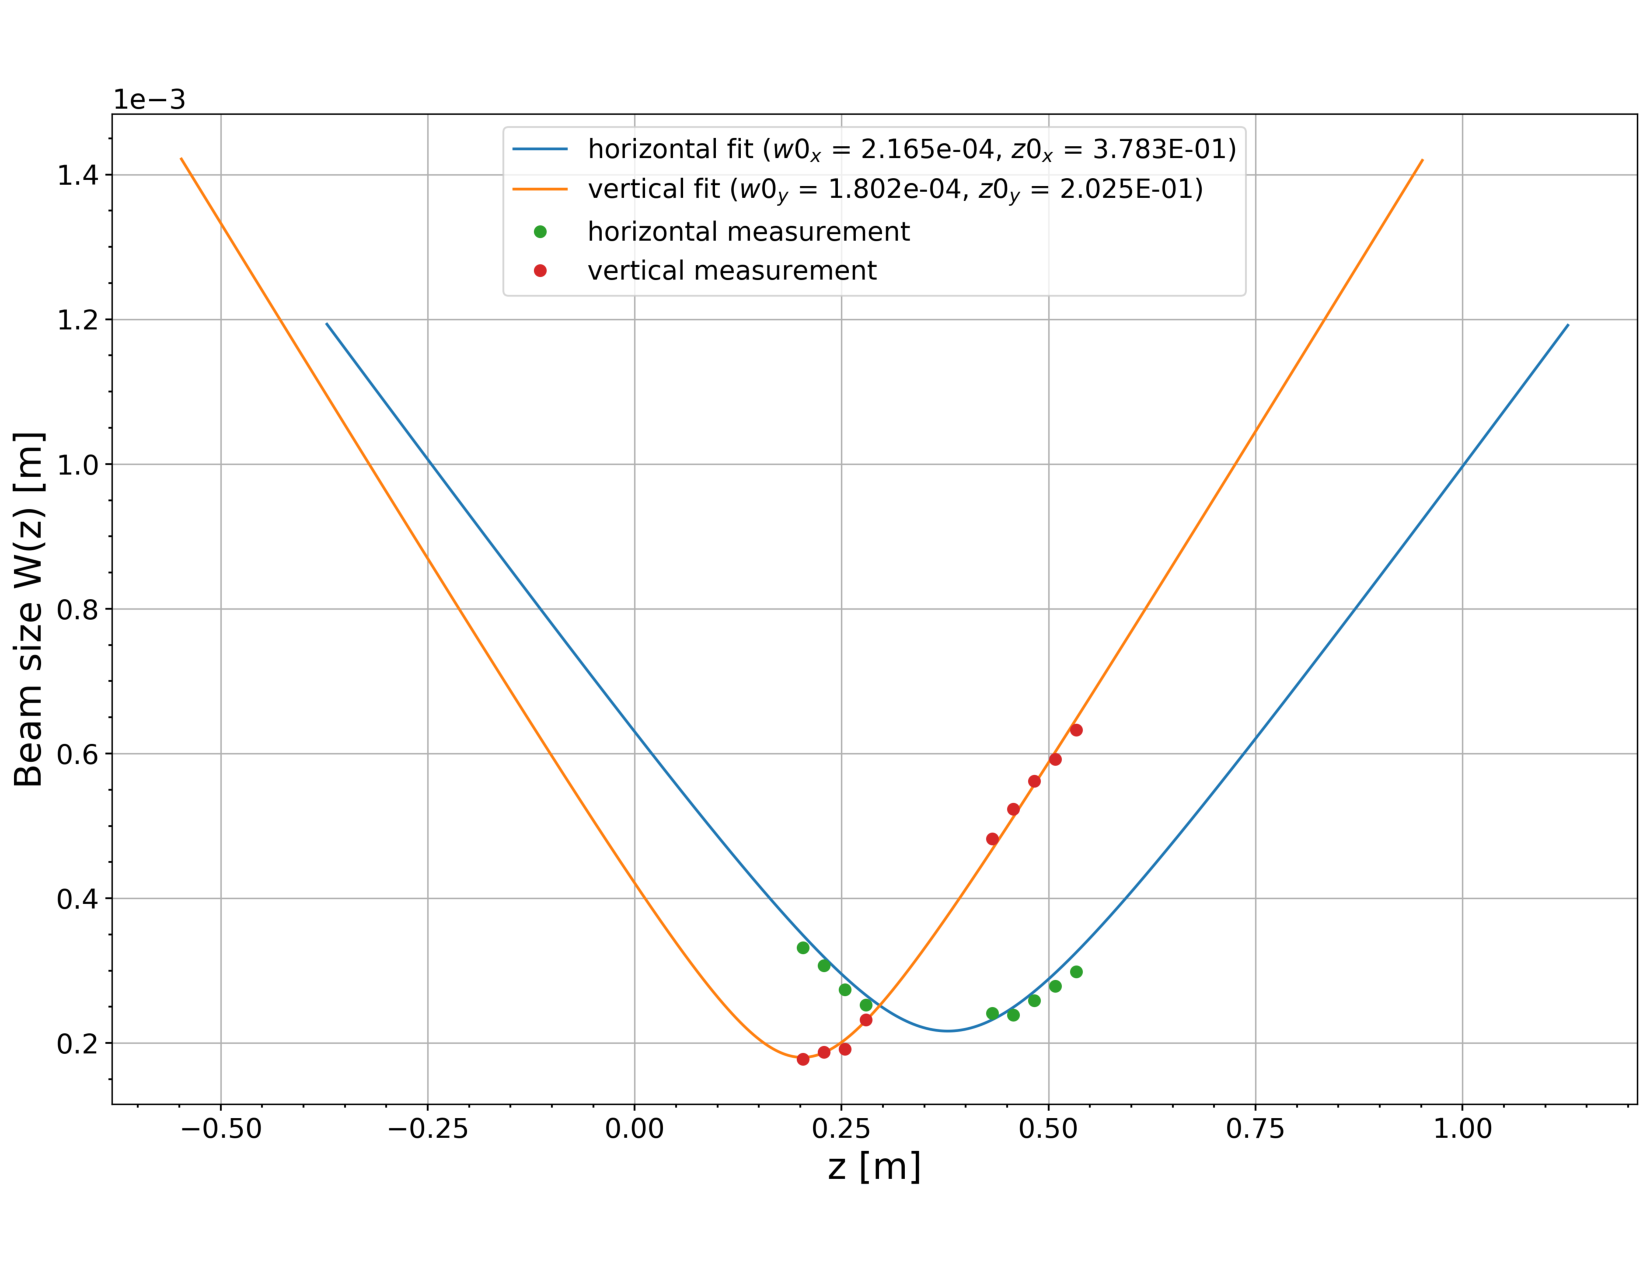
\includegraphics[width=\textwidth]{figs/ALGAAS/beam_scans/12_18_2020_preMMT.pdf}
\caption{\textcolor{red}{Figure of two mirror cavity}}
\label{fig:cav_stab}
\end{figure}

\section{Paraxial equation} \label{sec:paraxial}

The general three dimensional wave equation for an E-field $E(x,y,z,t)$ is provided by Maxwell:

$$ \label{eq:waveq}
	\bigg( \nabla ^2 + \frac{1}{c^2} \frac{\partial^2}{\partial t^2} \bigg) E(x,y,z,t) = 0
$$

For a coherent beam ($k = \frac{2 \pi}{\lambda}$), we analyze the purely spatial component of the solution and select a longitudinal propogation ($\vec{z}$) direction such that our solution will look like the following (utilizing Helmholtz's equation):

$$
	E(x,y,z) = E_0(x,y,z) e^{-ikz}
$$

The above wavefunction combined with Helmoltz equation requires that complex form of $E_0$ obeys the paraxial equation:

\begin{equation}\label{eq:paraxial}
	\bigg( \frac{\partial^2}{\partial x ^2} + \frac{\partial^2}{\partial y^2} - 2ik \frac{\partial}{\partial z} \bigg) E_0(x,y,z) = 0
\end{equation}

\section{The Equipartition theorem and the Fluctuation dissapation theorem}

\section{Monochromatic plane wave propogation}
Revisiting Maxwell's equations for a simple monochromatic plane wave solution provides further direction on how crystalline media may effect incident light. Further elaborating, the following assumptions are made:
\begin{equation}
\vec{E} = E_o e^{(i \omega (\frac{n}{c} \vec{r}\cdot \vec{s}-t))}
\end{equation}
Where $n$ is the index of refraction, $c$ is the speed of light, $\vec{r}$ is the position vector and $\vec{s}$ is the unit wave normal.
\begin{equation}
\nabla \times \vec{H}= \frac{\partial \vec{D}}{\partial t}
\end{equation}
Where $\vec{H}$ is the magnetic field assuming permeability $\mu$, and the generalized displacement vector $\vec{D}$ and electric field vector $\vec{E}$.
\begin{equation}
\nabla \times \vec{E} = -\mu \vec{H}
\end{equation}
Reducing to only the displacement and electric fields:
\begin{equation}\label{eq:dispelec}
\vec{D} = \frac{n^2}{\mu}[\vec{E}-\vec{s}(\vec{s}\cdot \vec{E})]
\end{equation}
Maxwell's equations show that the electric field is not necessarily parallel to the displacement field and in most materials with non-zero polarizability tensors and dielectric tensors, it is not. But as specified above, the displacement vector, Electric field and unit wave normal are co-planar while remaining orthogonal to $\vec{H}$. Assuming we are operating within a coordinate system aligned with the principal dielectric axes, we substitute \autoref{eq:dispfield} into \autoref{eq:dispelec}:
\begin{equation}
E_i = \frac{n^2 s_i (\vec{E}\cdot\vec{s})}{n^2 - \mu \varepsilon_i}
\end{equation}

From here it can be shown that for a general plane wave there exist two unique refractive index solutions within the constructed dielectric ~\cite{nye}. 

\newpage

\section{Thermo-optic filters}

\subsection{COMSOL self heating filter}
\begin{figure}[H]
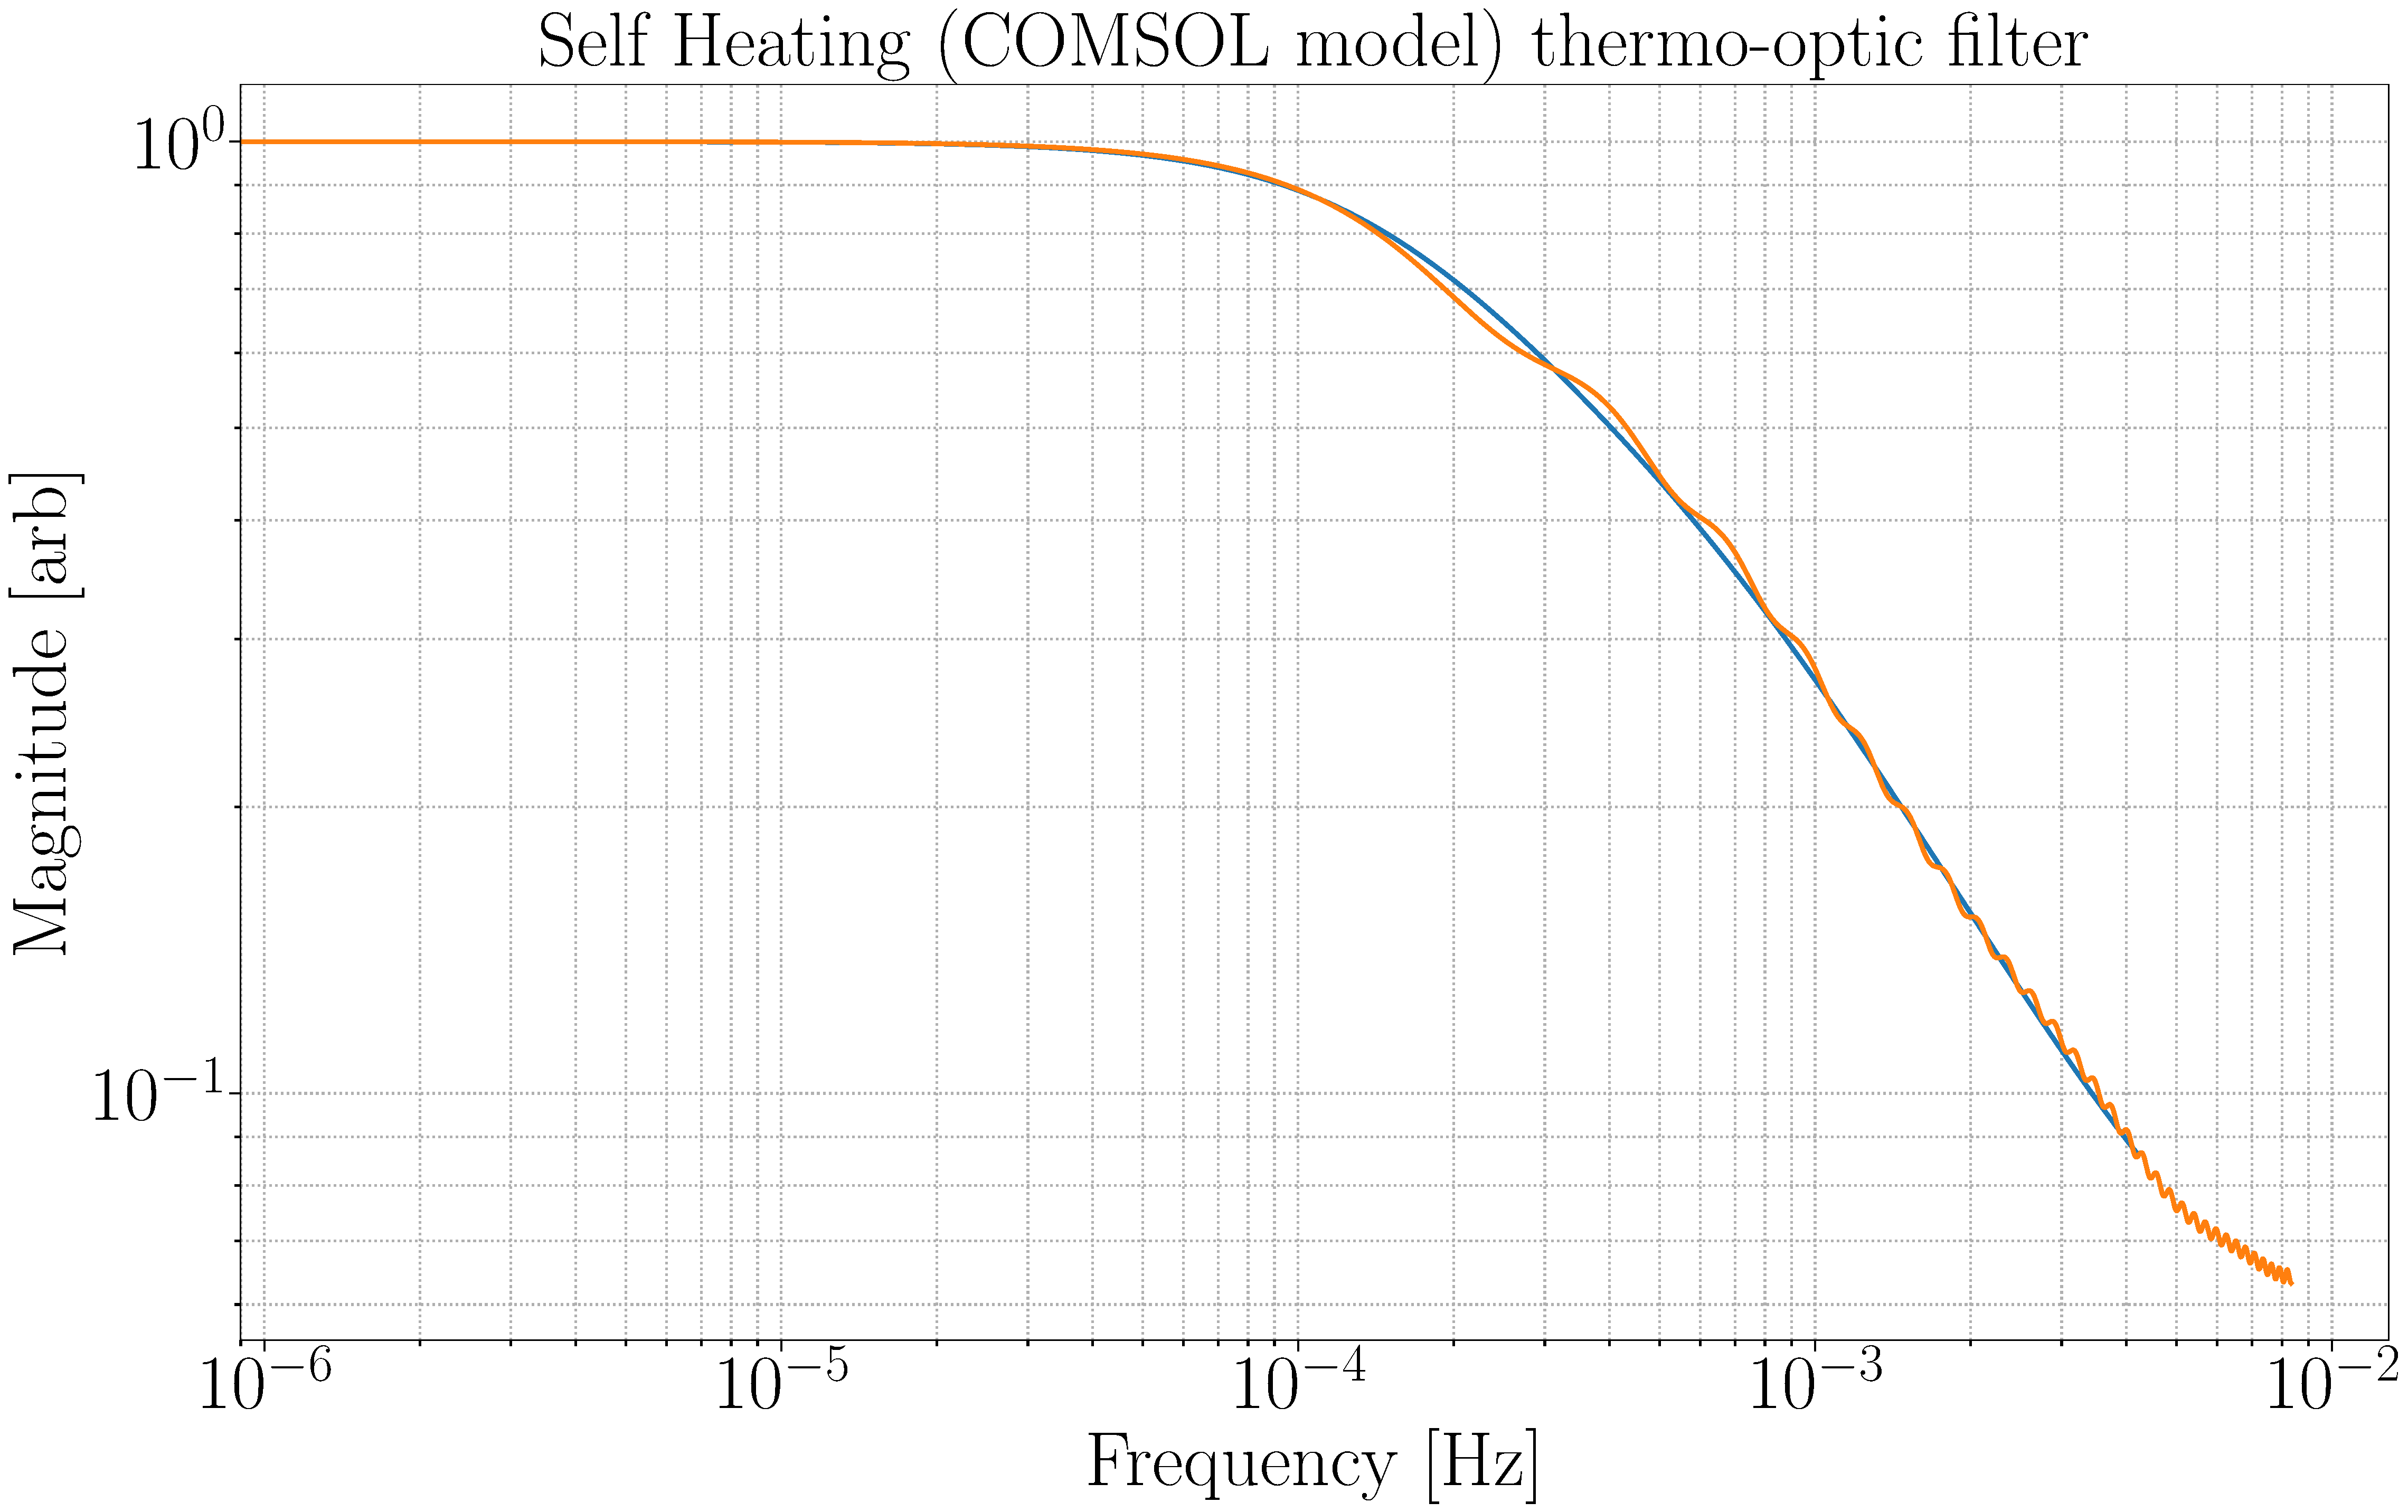
\includegraphics[width=\textwidth]{figs/TCS/self_heating_zpk.pdf}
\caption{Fitted zpk filter to transient response of self heating COMSOL model.}
\label{fig:self_zpk_fit}
\end{figure}

\subsection{RH filter}


\subsection{CO2 filter}
\begin{figure}[H]
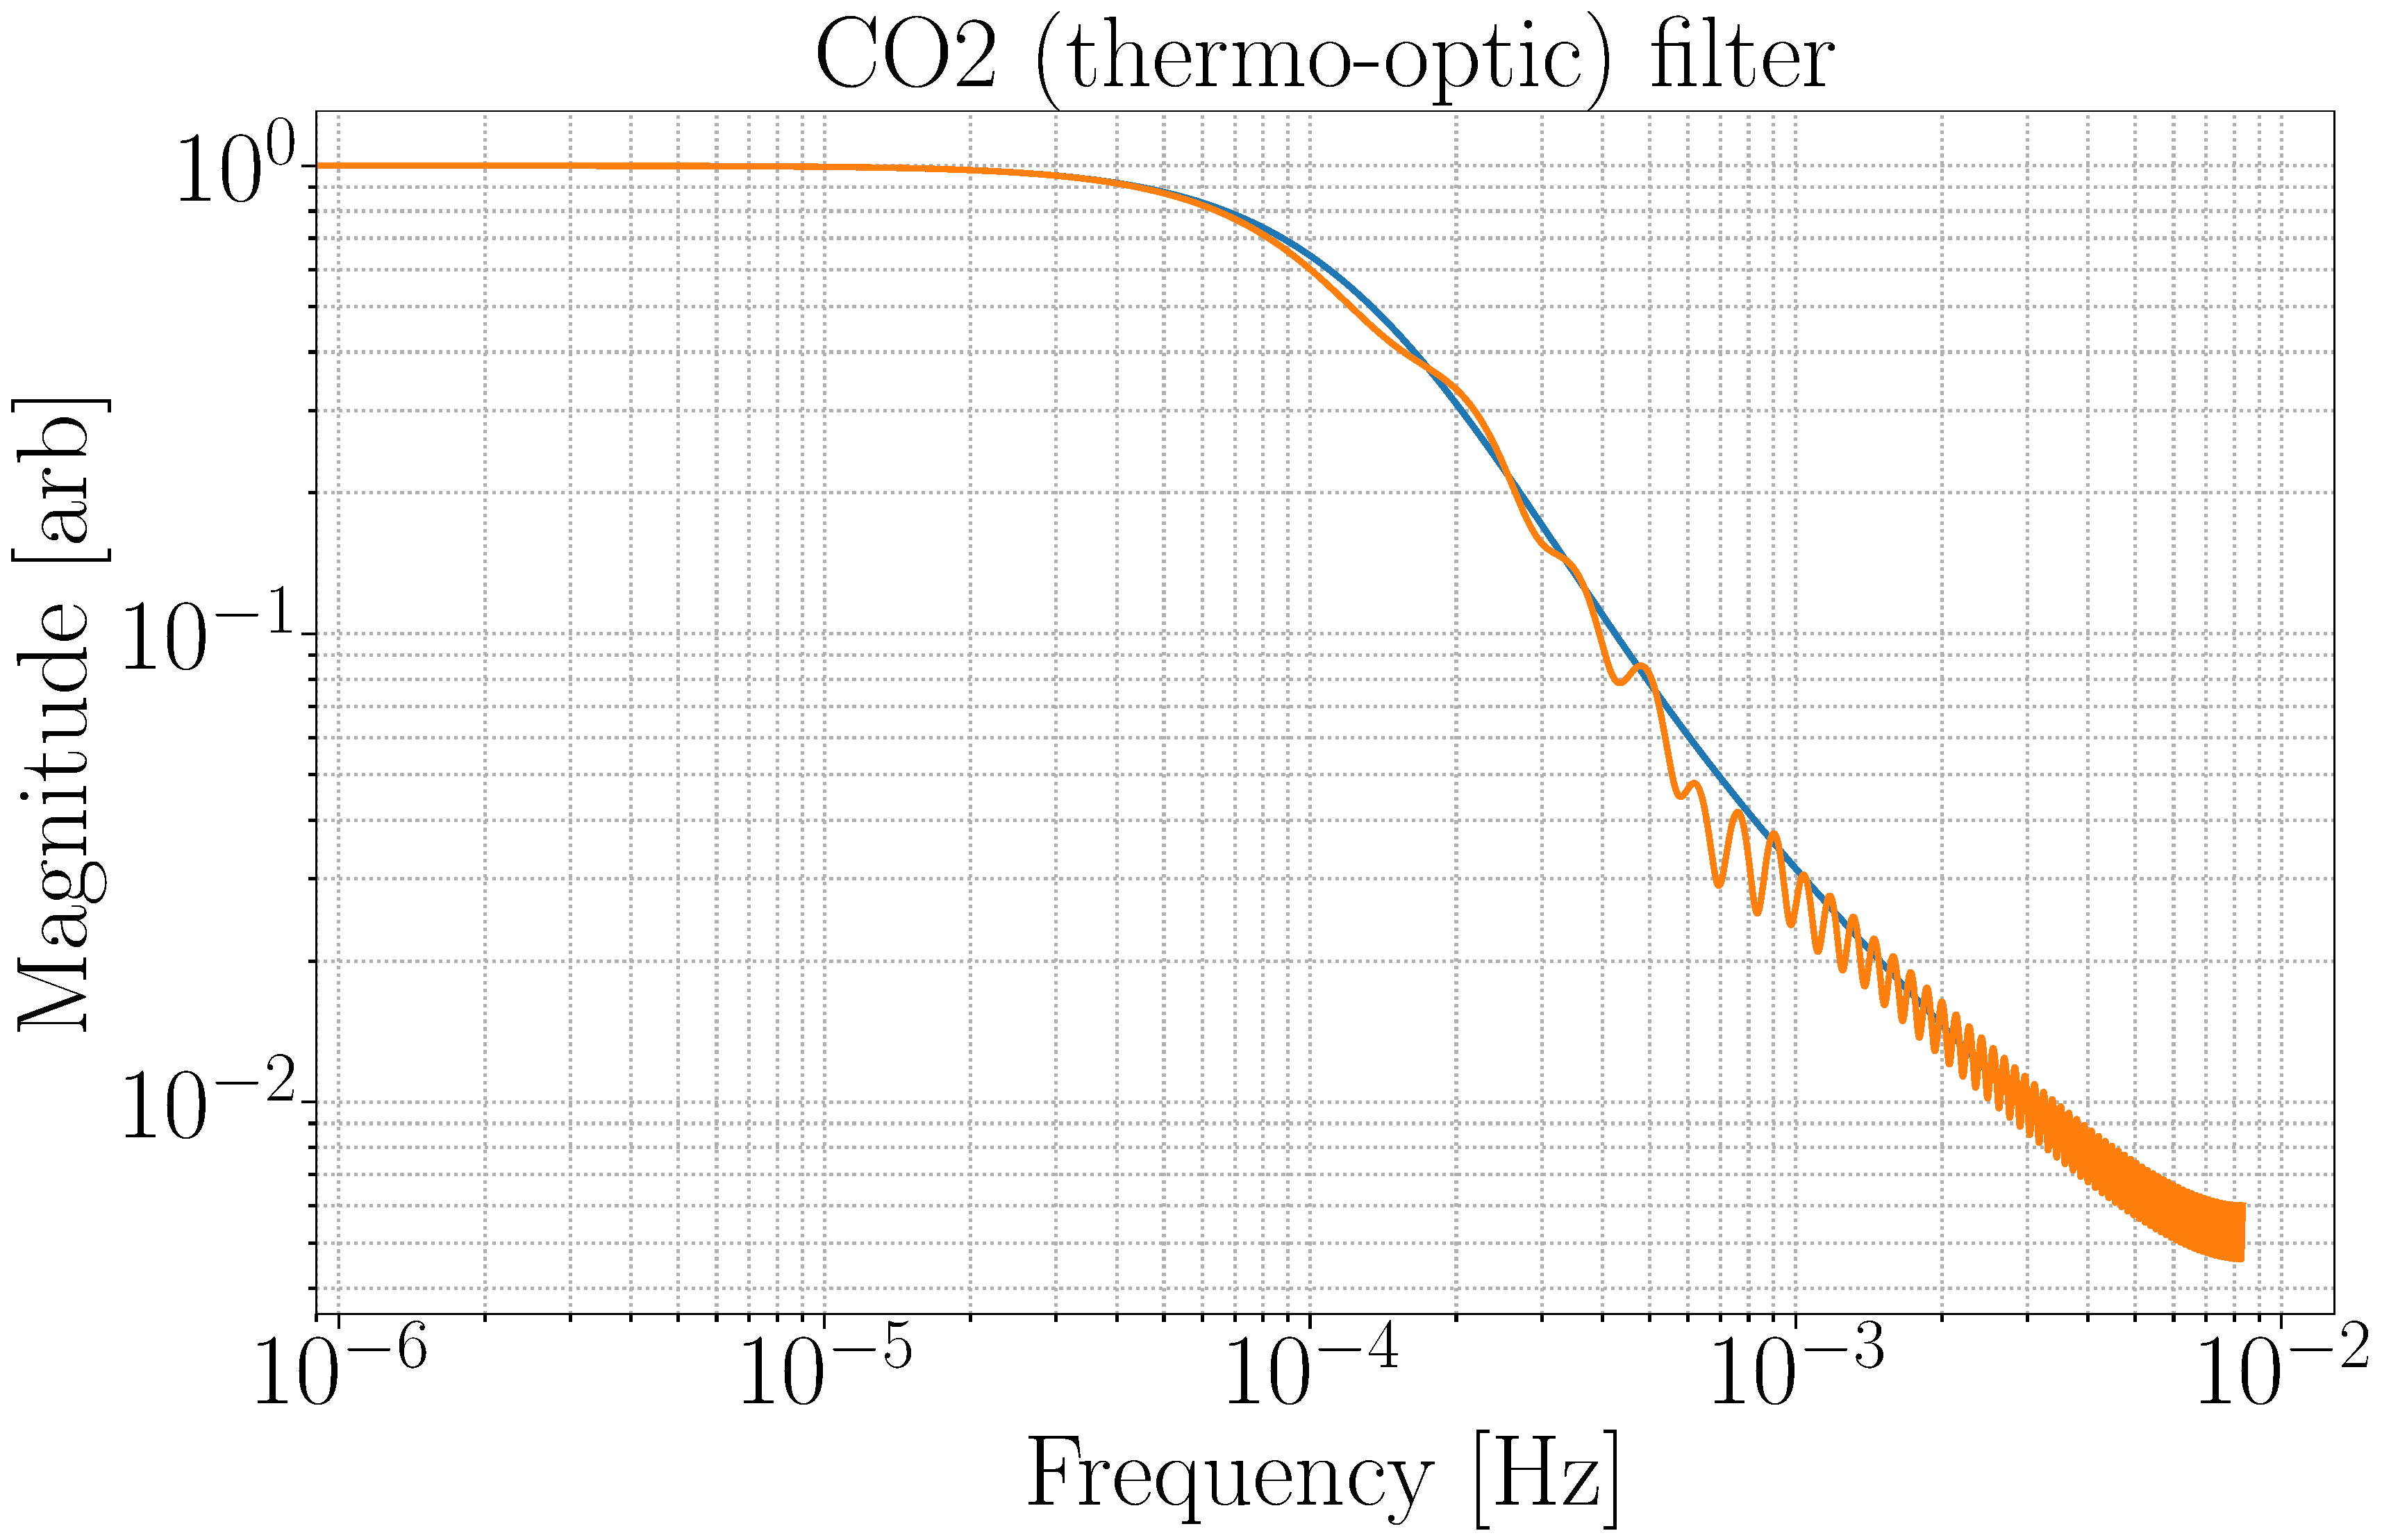
\includegraphics[width=\textwidth]{figs/TCS/CO2_zpk.pdf}
\caption{Fitted zpk filter to transient CO2 actuation response.}
\label{fig:co2_zpk_fit}
\end{figure}

\section{Mode matching data for Electro-optic sample cavity}

\subsection{Pre MMT beam scan}

\begin{figure}[H]
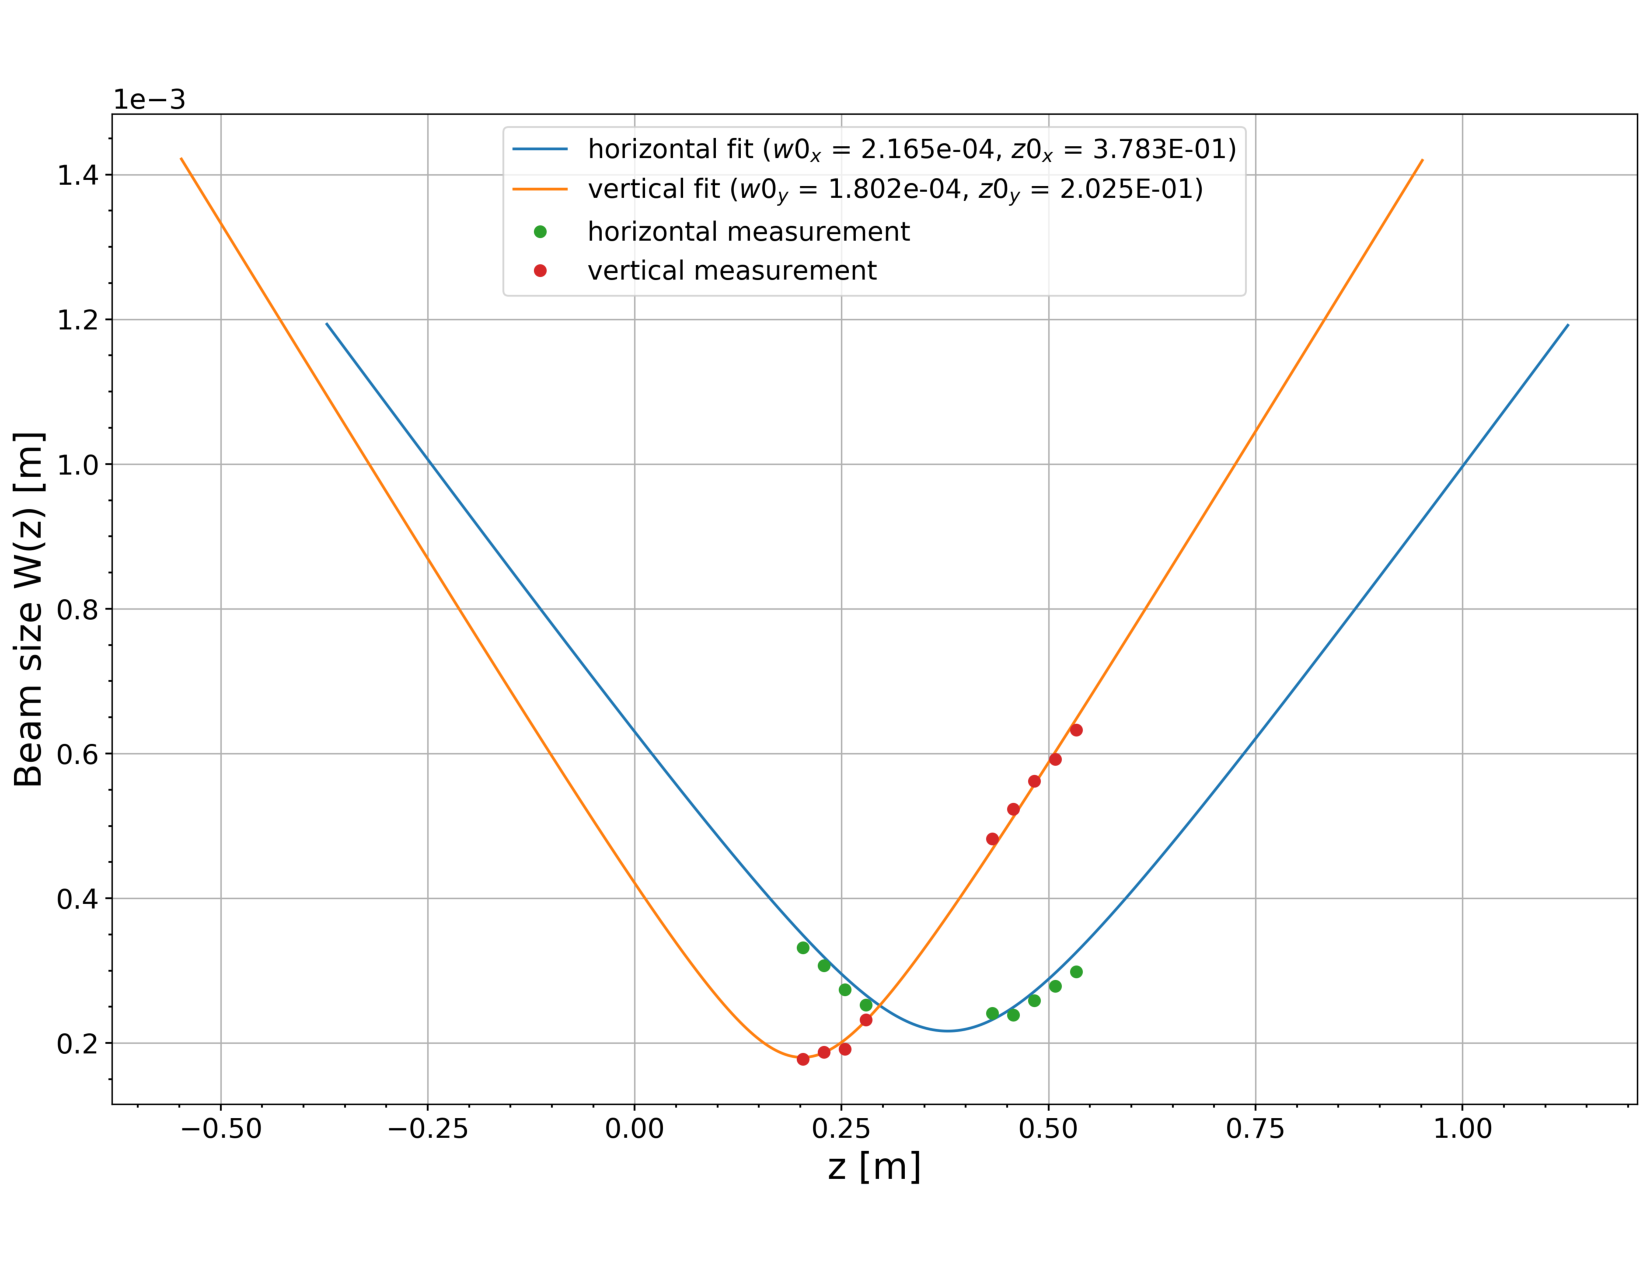
\includegraphics[width=\textwidth]{figs/ALGAAS/beam_scans/12_18_2020_preMMT.pdf}
\caption{Beam scan taken from SM5 (Steering mirror 5)}
\label{fig:beamscan2020}
\end{figure}


\subsection{``Just another mode matching tool" (JAMMT) solution}
\subsection{Post MMT beam scan}

\begin{figure}[H]
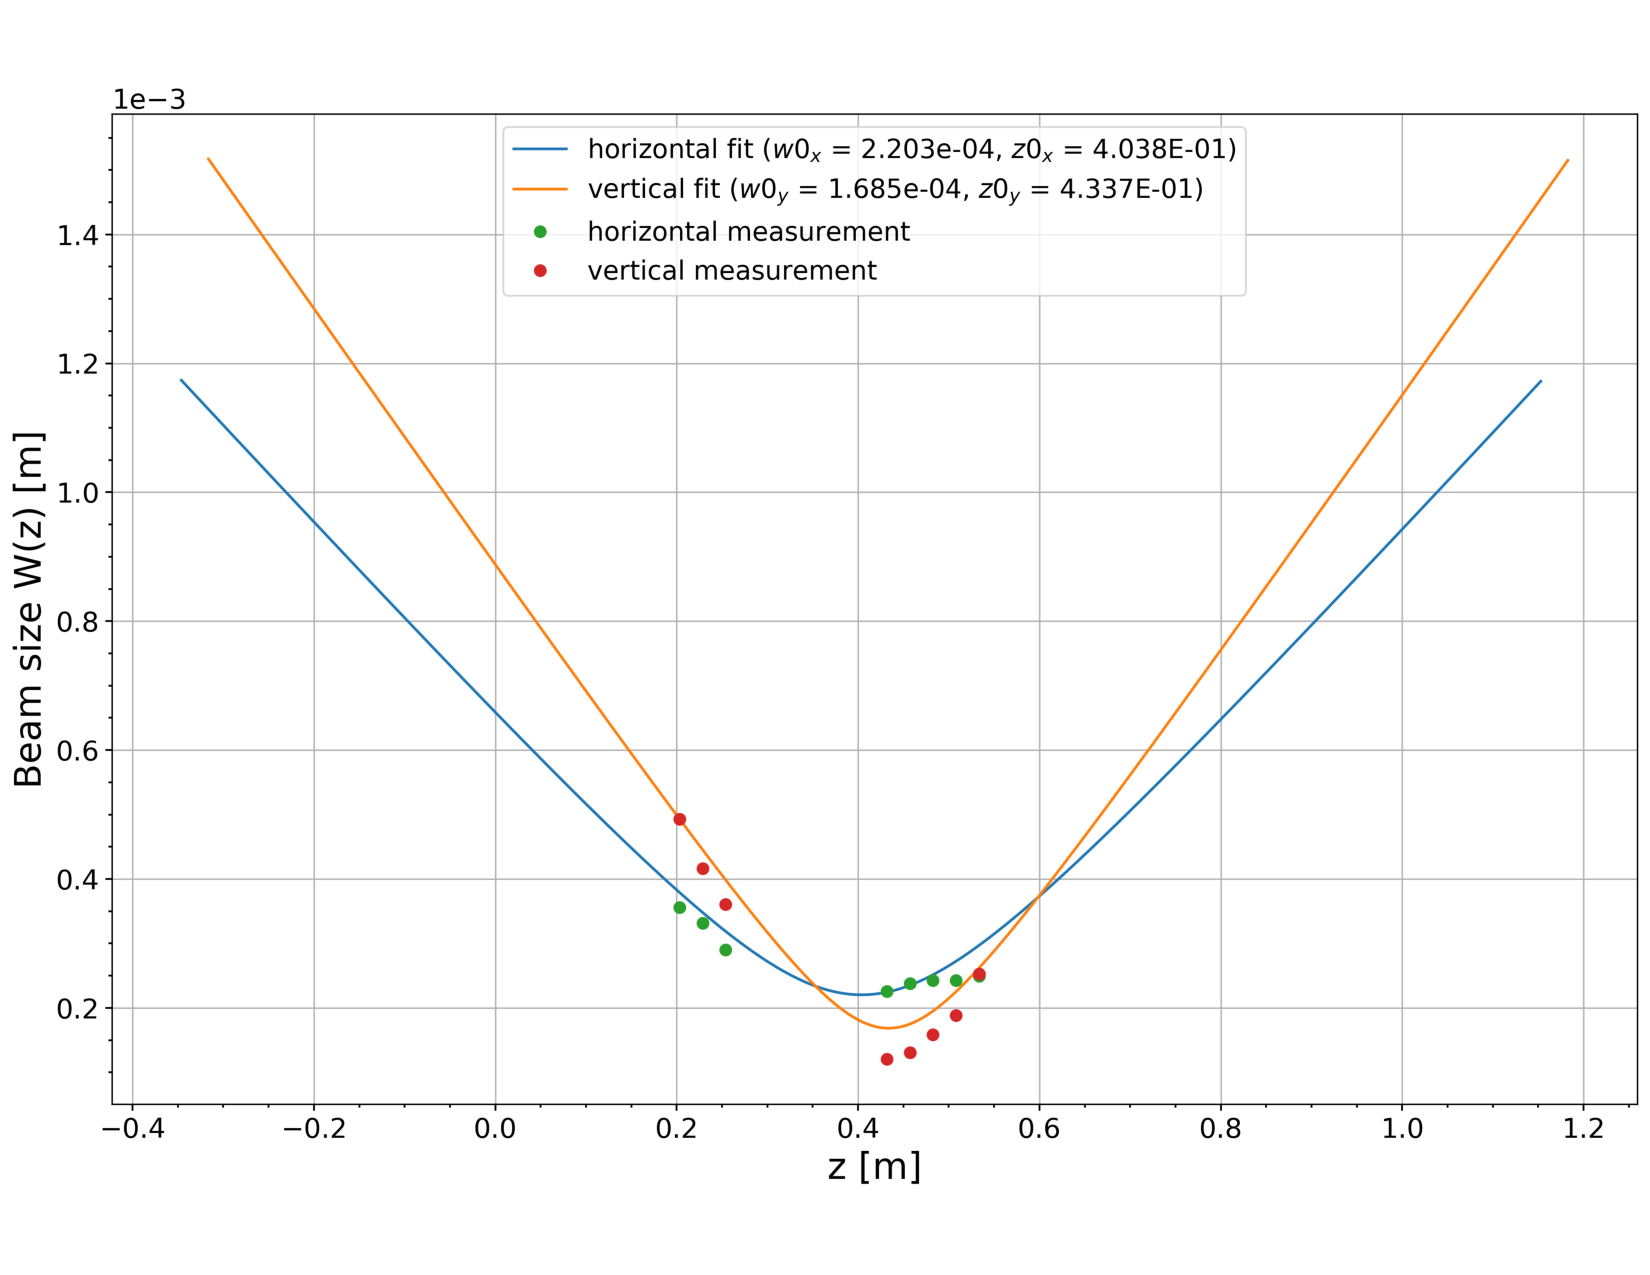
\includegraphics[width=\textwidth]{figs/ALGAAS/beam_scans/01_12_2021_postMMT.pdf}
\caption{Beam scan taken from SM6. Sampling points before SM7 and after the first cavity iris.}
\label{fig:beamscan2021}
\end{figure}

\subsection{Laser PZT sweep}

\begin{figure}[H]
	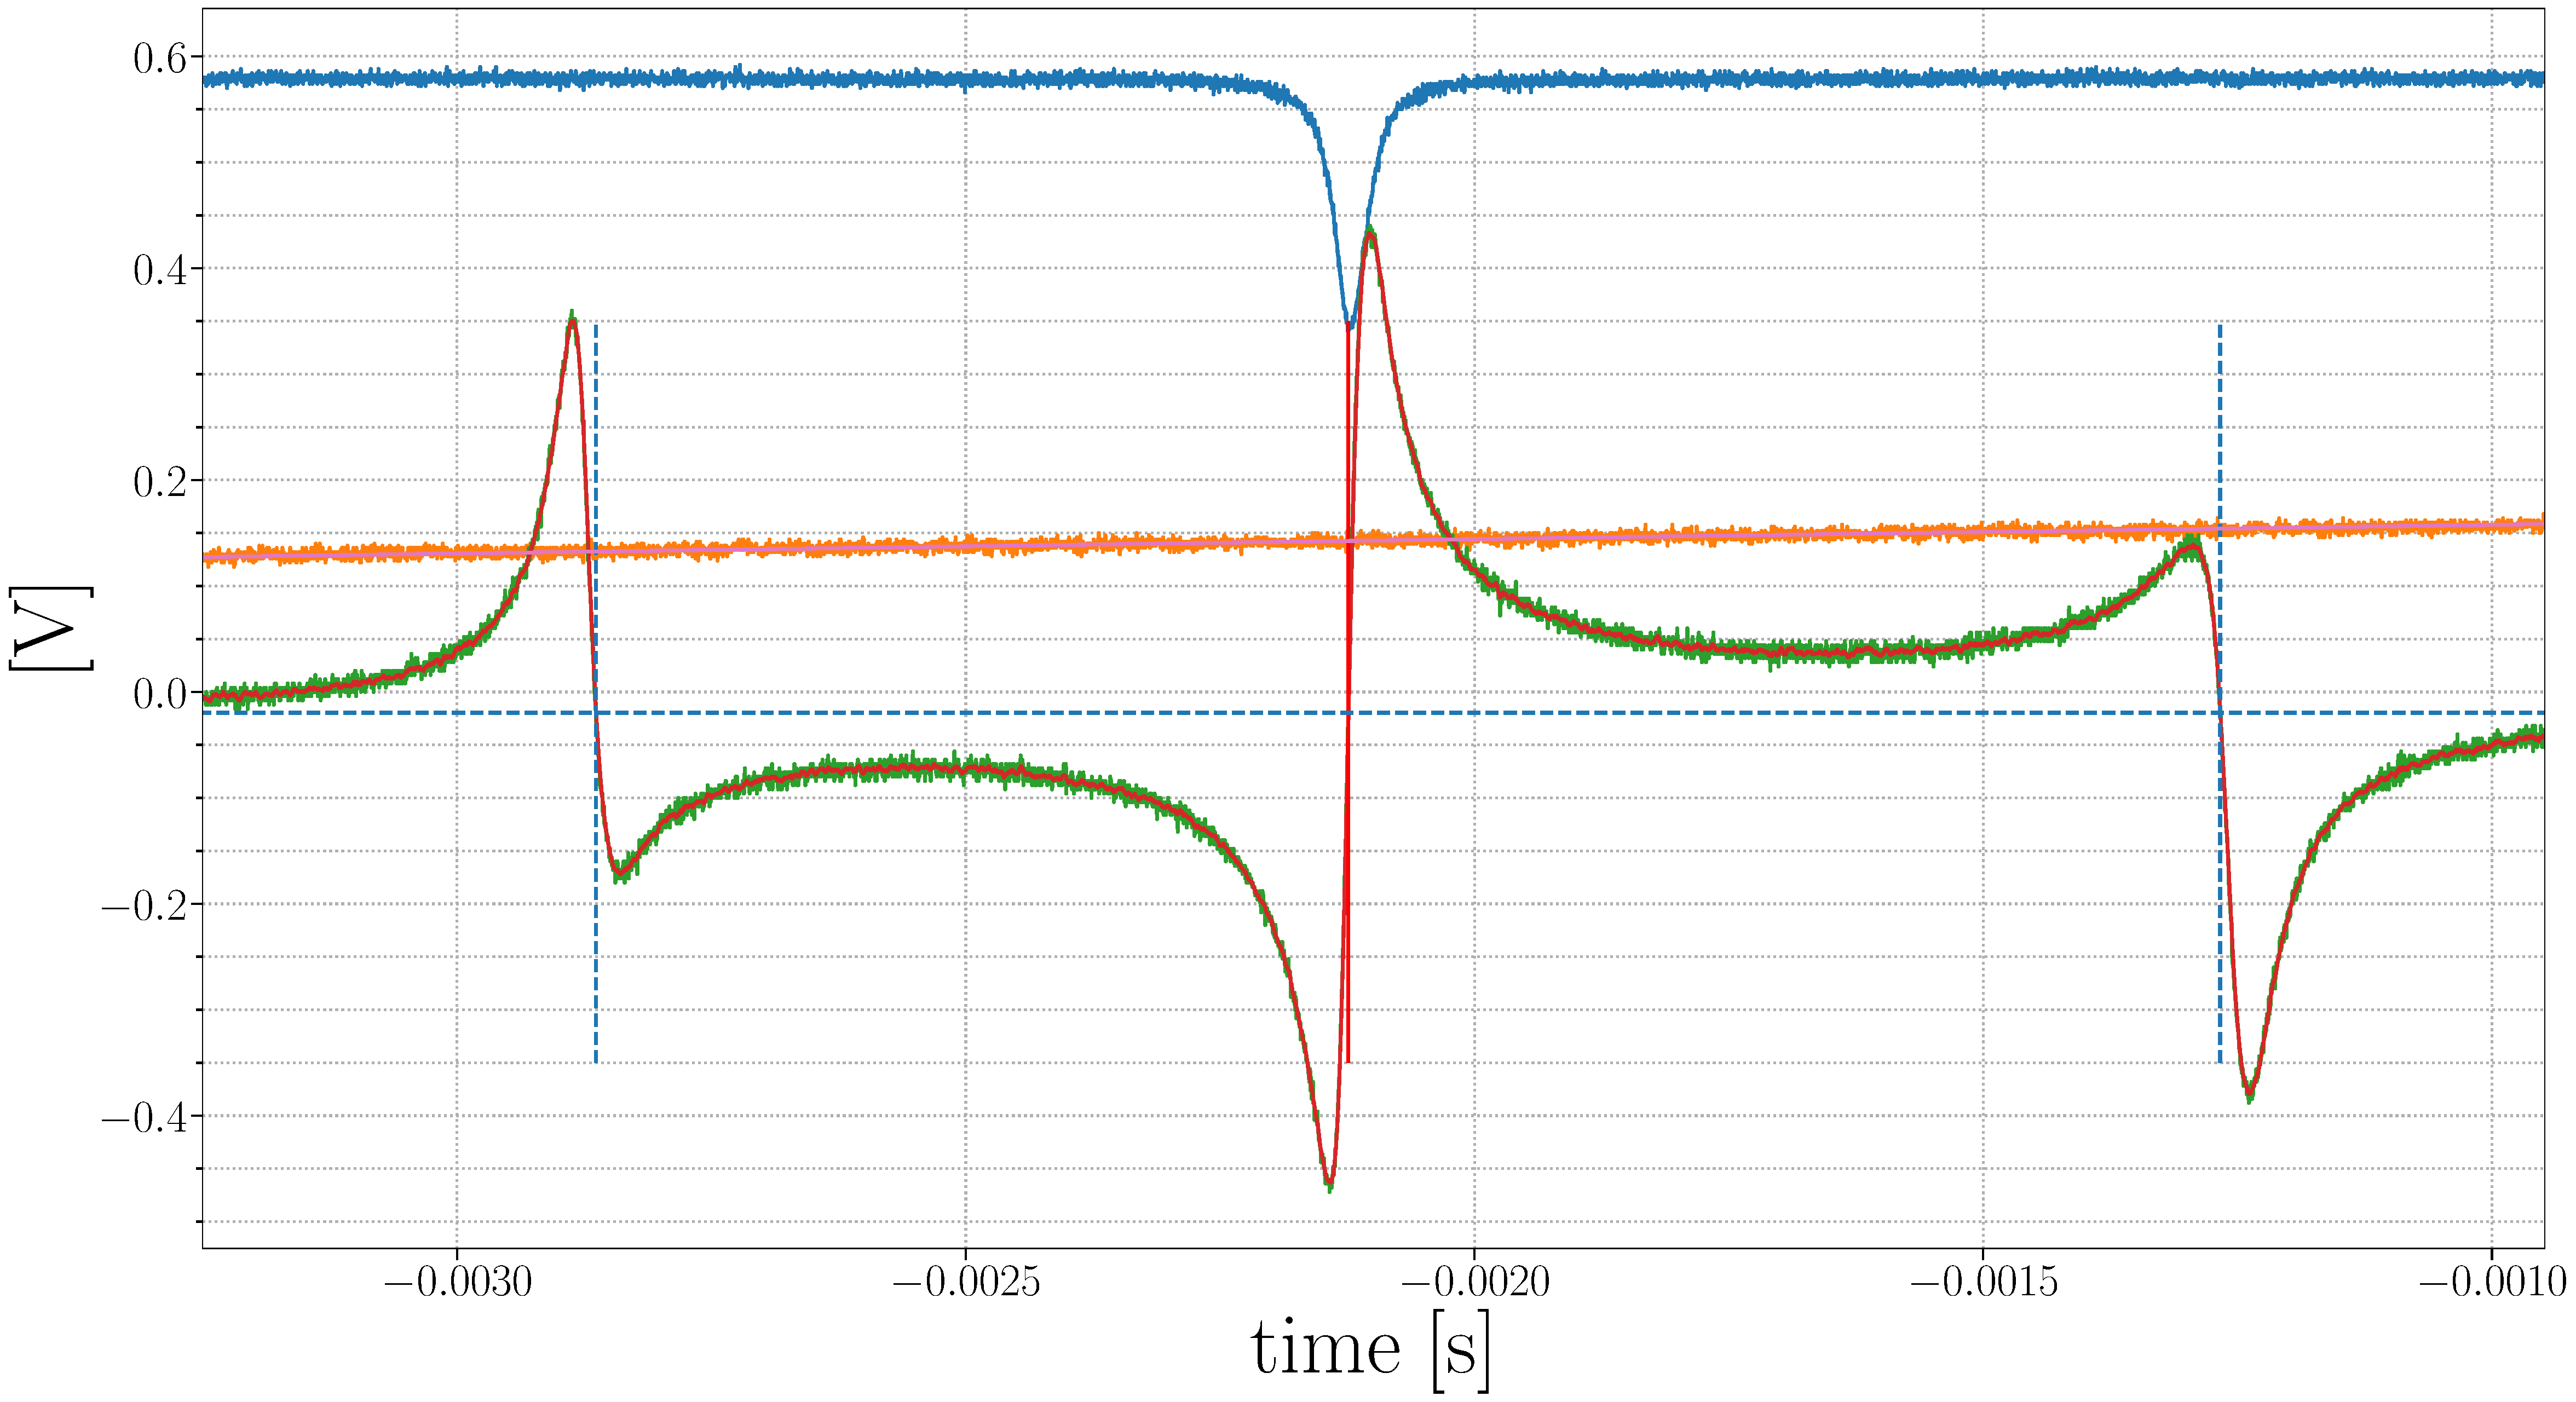
\includegraphics[width=\textwidth]{figs/ALGAAS/pdh_measured.pdf}
	\caption{Ramping voltage sent to the laser PZT while probing the mixer output. The sweep was performed for sample cavity of length notes}
\label{fig:pdhmeasured}
\end{figure}

\newpage

\section{Assembly blueprints and alternative views}

\subsection{Assembly 1}

\subsubsection{Cross section}

\subsubsection{Electrodes}

\subsubsection{Iteration 1.1}

\begin{figure}[!ht]
	\begin{subcaptiongroup}
		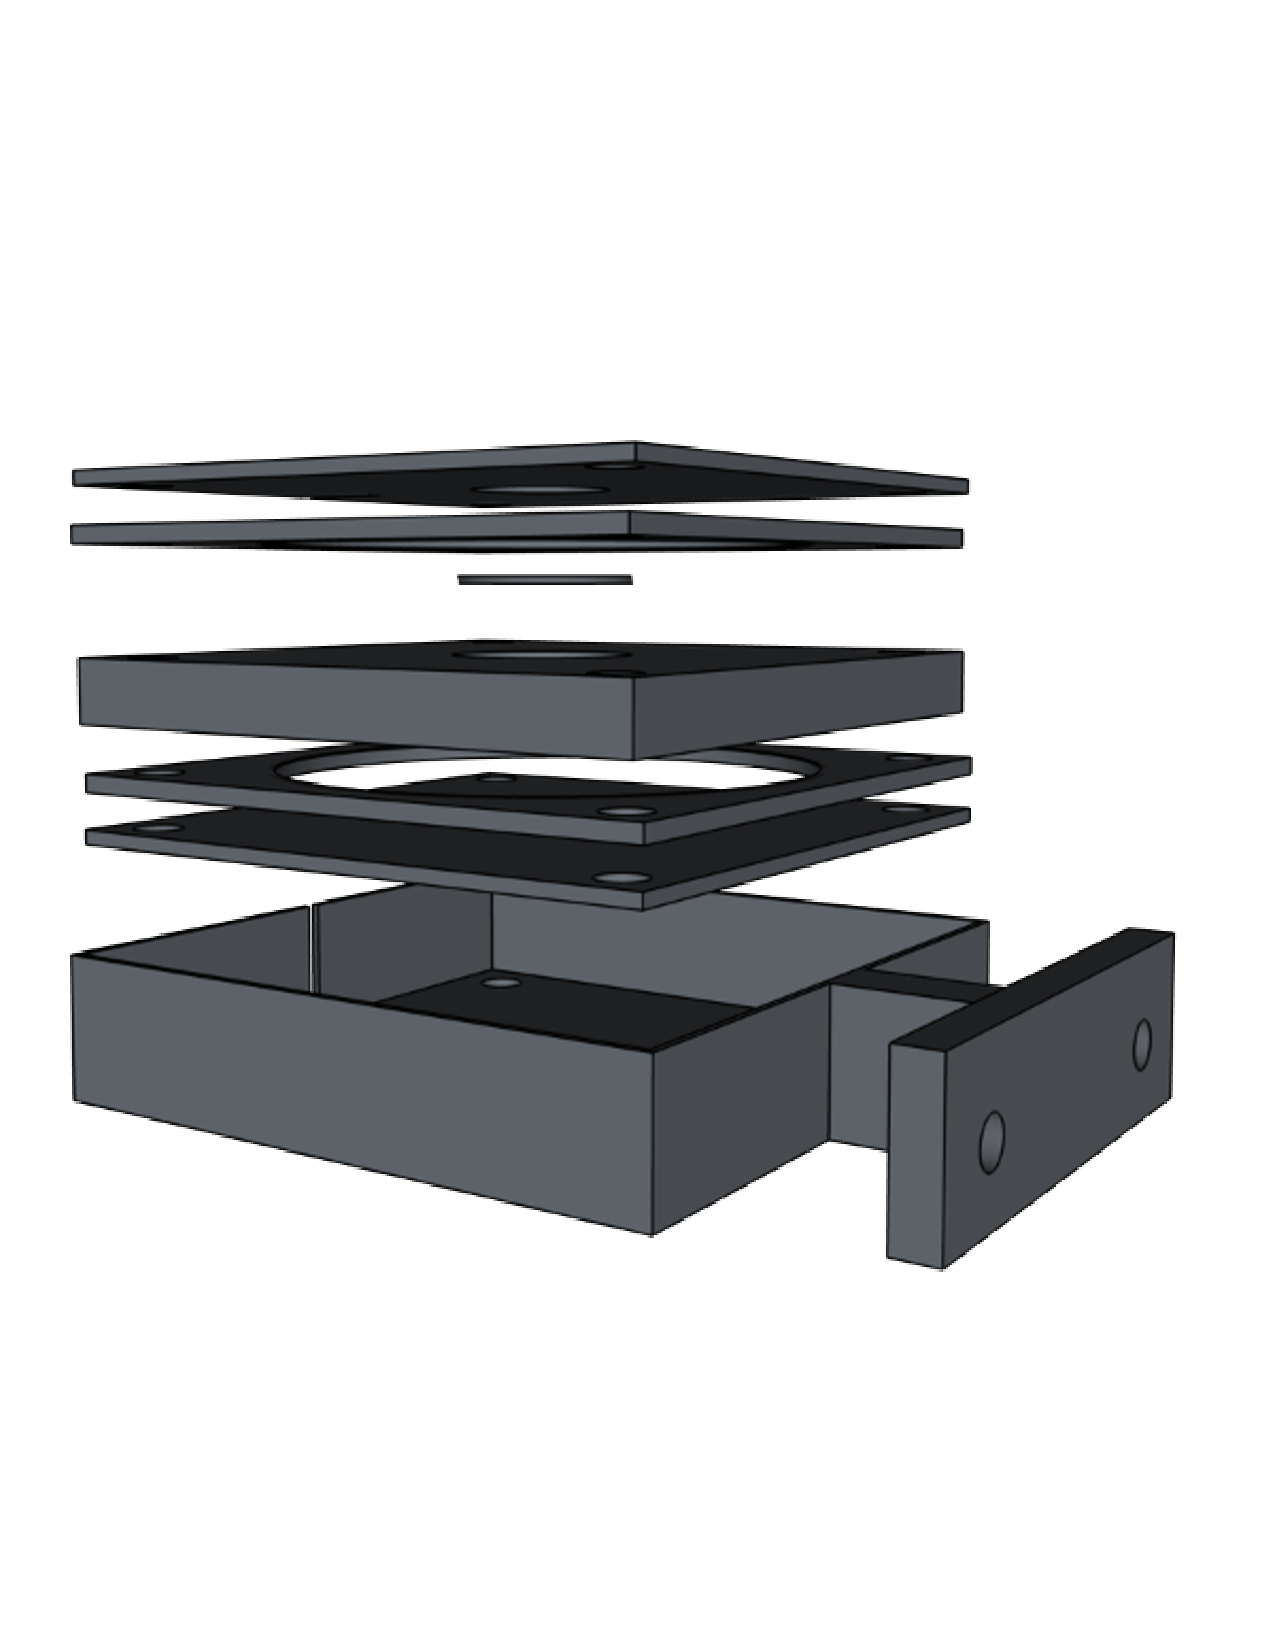
\includegraphics[width=.5\textwidth]{figs/ALGAAS/assemblies/assembly0/assembly0.pdf}
		\phantomcaption\label{A0}
		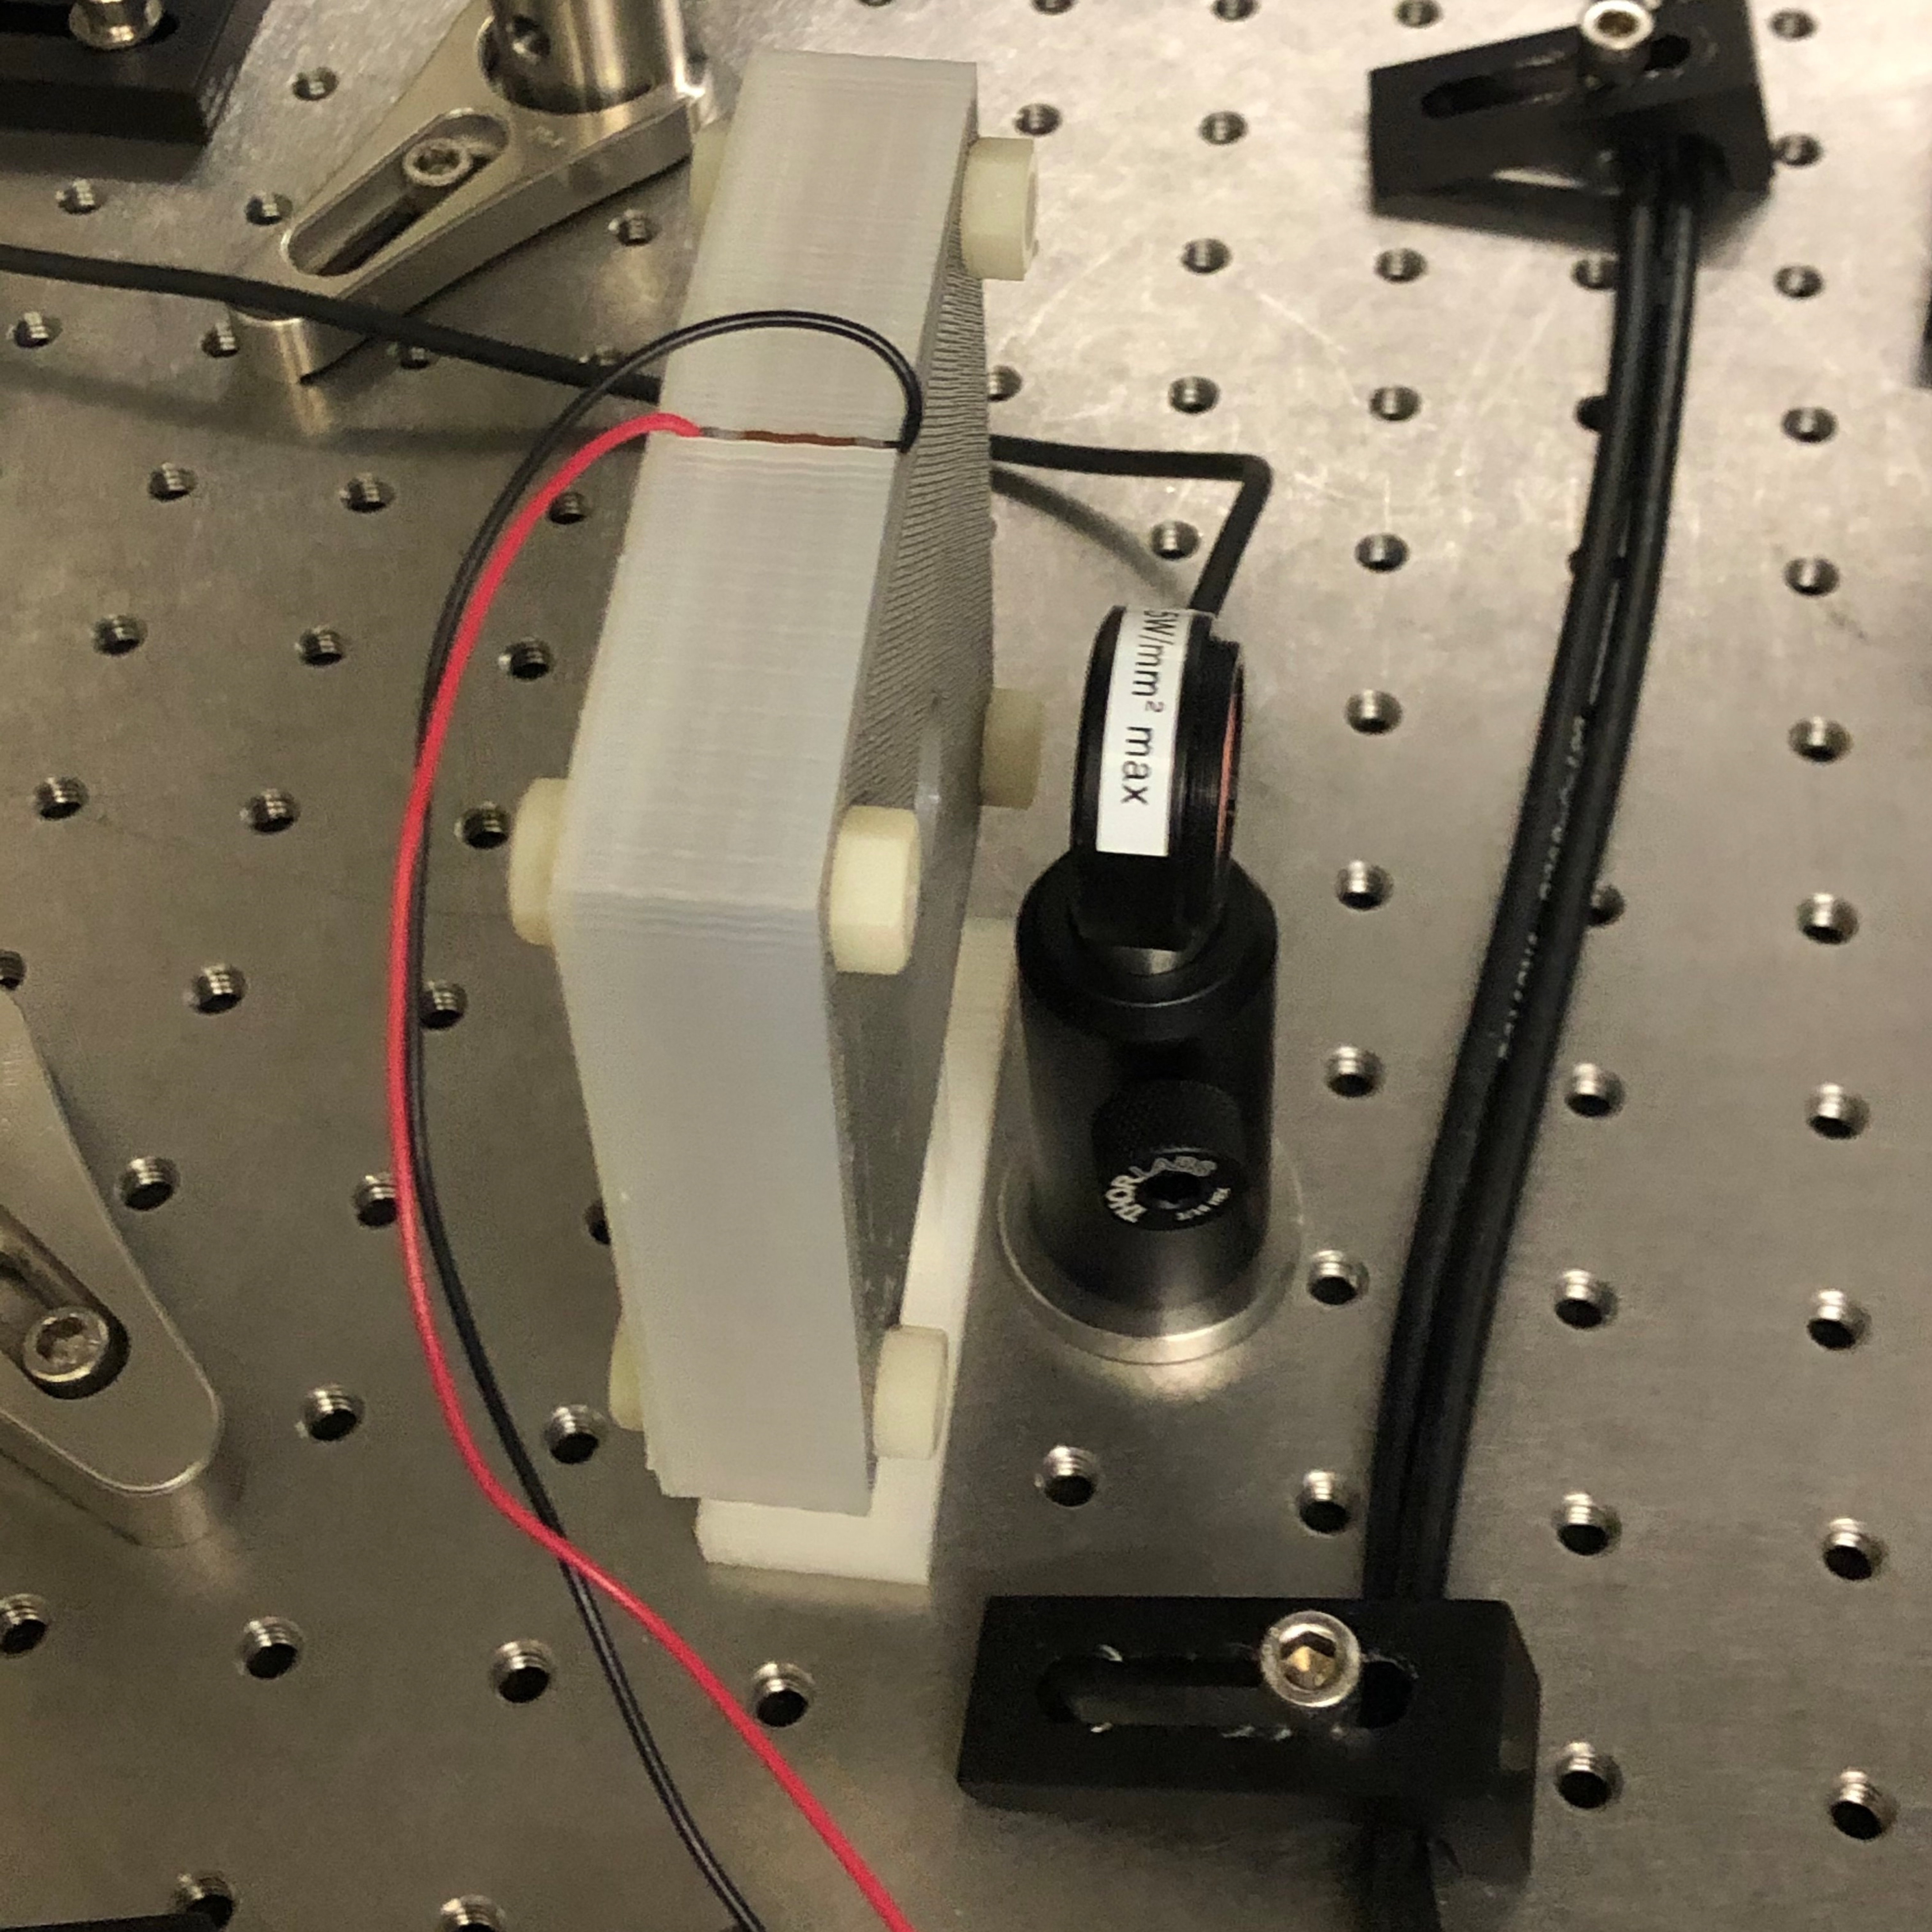
\includegraphics[width=.5\textwidth]{figs/ALGAAS/assemblies/assembly0/assembly0_incident_power.pdf}
 		\phantomcaption\label{A0inc}
	\end{subcaptiongroup}
  \caption{Assembly 0 was constructed to meet the criteria of providing a non-conductive housing for the electrode / sample assembly while maintaining a fixed length spacing using parts 3d printed with polylactic acid (PLA).}
  \label{fig:assembly0bp}
\end{figure}
\FloatBarrier

\subsubsection{Iteration 1.2}
\begin{figure}[!ht]
	\begin{subcaptiongroup}
		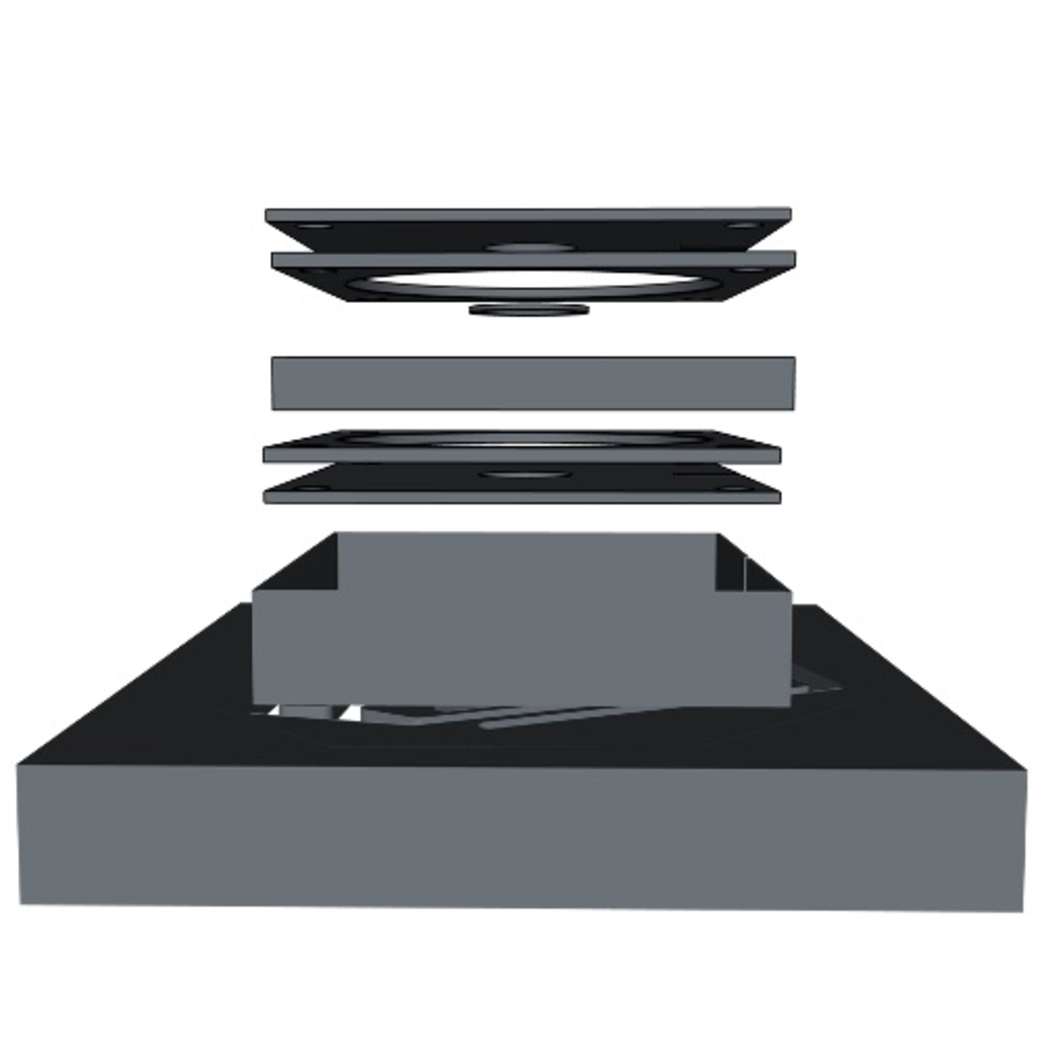
\includegraphics[width=.5\textwidth]{figs/ALGAAS/assemblies/assembly1/assembly1_dissassembled.pdf}
		\phantomcaption\label{A1pt2CAD}
		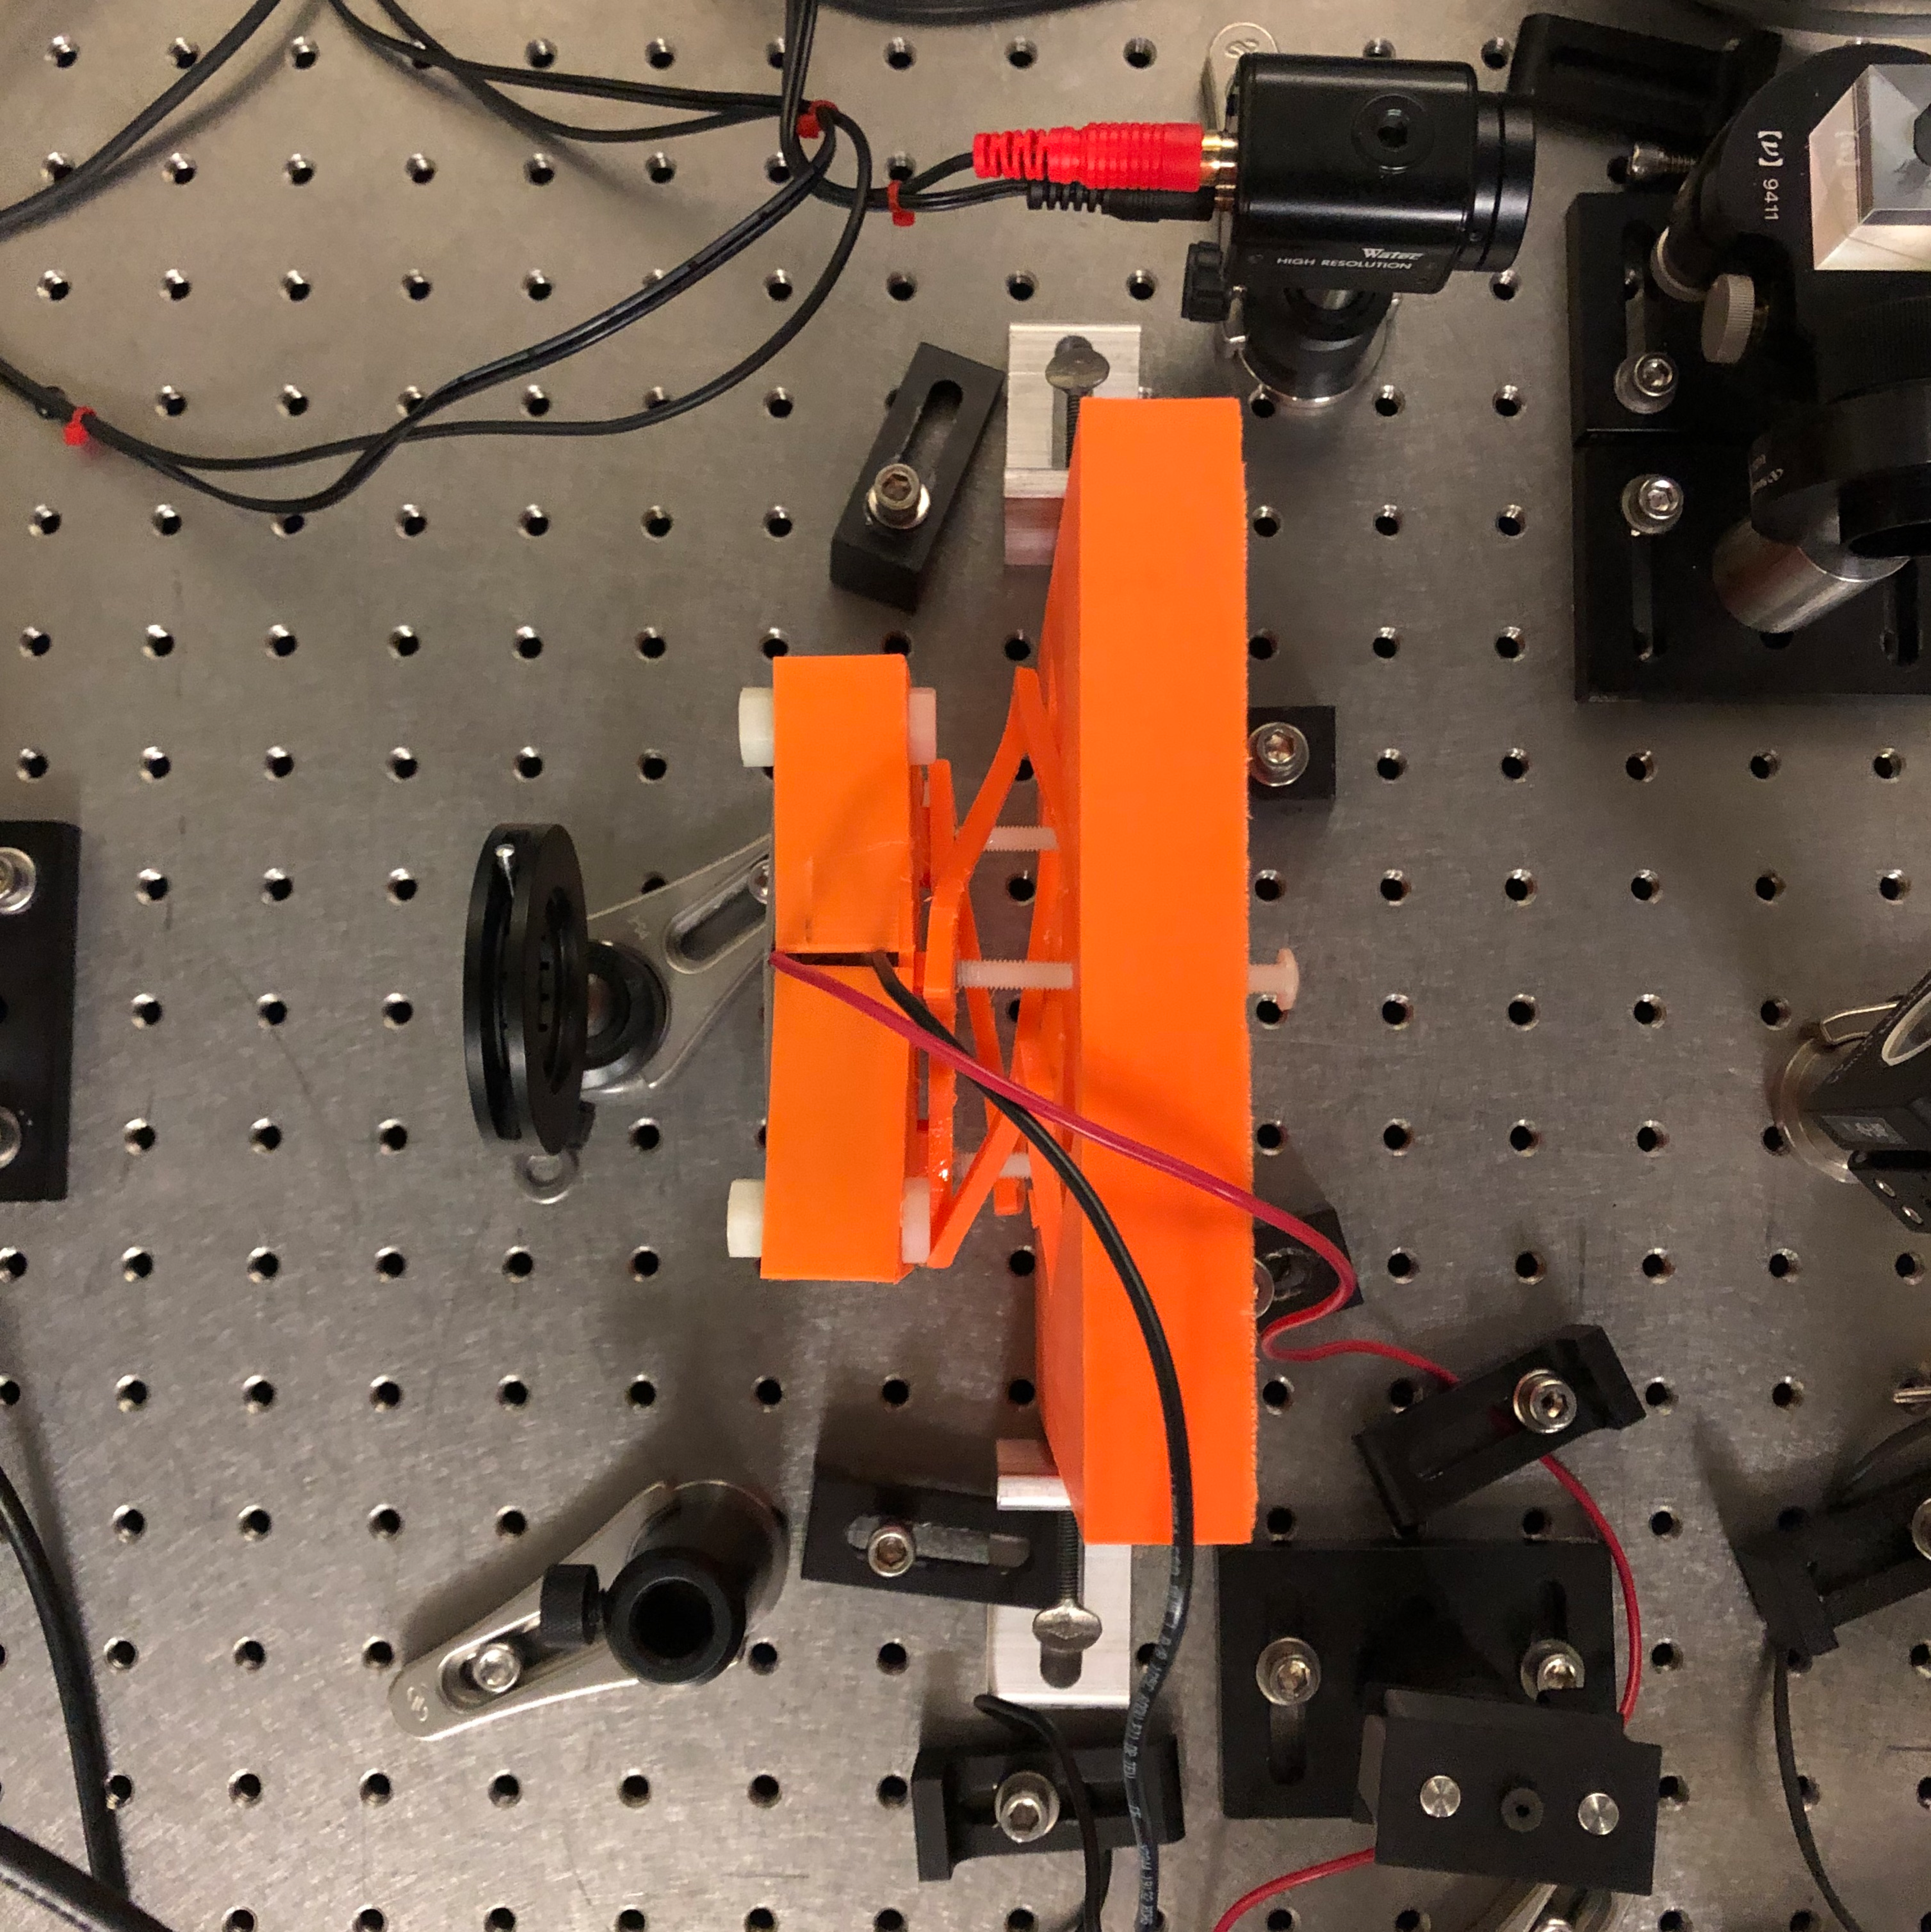
\includegraphics[width=.5\textwidth]{figs/ALGAAS/assemblies/assembly1/assembly1_insitu2.pdf}
		\phantomcaption\label{A1pt2pic}	
	\end{subcaptiongroup}
	\caption{Assembly 1 was constructed to meet the criteria of providing a non-conductive housing for the electrode / sample assembly while maintaining a fixed length spacing using parts 3d printed with polylactic acid (PLA).}
	\label{fig:assembly1bp}
\end{figure}
\FloatBarrier

\subsubsection{Iteration 1.3}
\begin{figure}[!ht]
	\begin{subcaptiongroup}
		\includegraphics[width=.5\textwidth]{figs/ALGAAS/assemblies/assembly1/assembly1_mod_front.pdf}
		\phantomcaption\label{A1pt3CAD}
		\includegraphics[width=.5\textwidth]{figs/ALGAAS/assemblies/assembly1/assembly1_mod_side.pdf}
		\phantomcaption\label{A1pt3pic}
	\end{subcaptiongroup}
	\caption{A modification implemented with the intention of reducing pitch dithering while still having control of DC YAW}
	\label{fig:assembly1mod}
\end{figure}

\newpage

\subsection{Assembly 2}
\subsubsection{Cross section}

\subsubsection{Electrodes}

\begin{figure}[H]
  \centering
  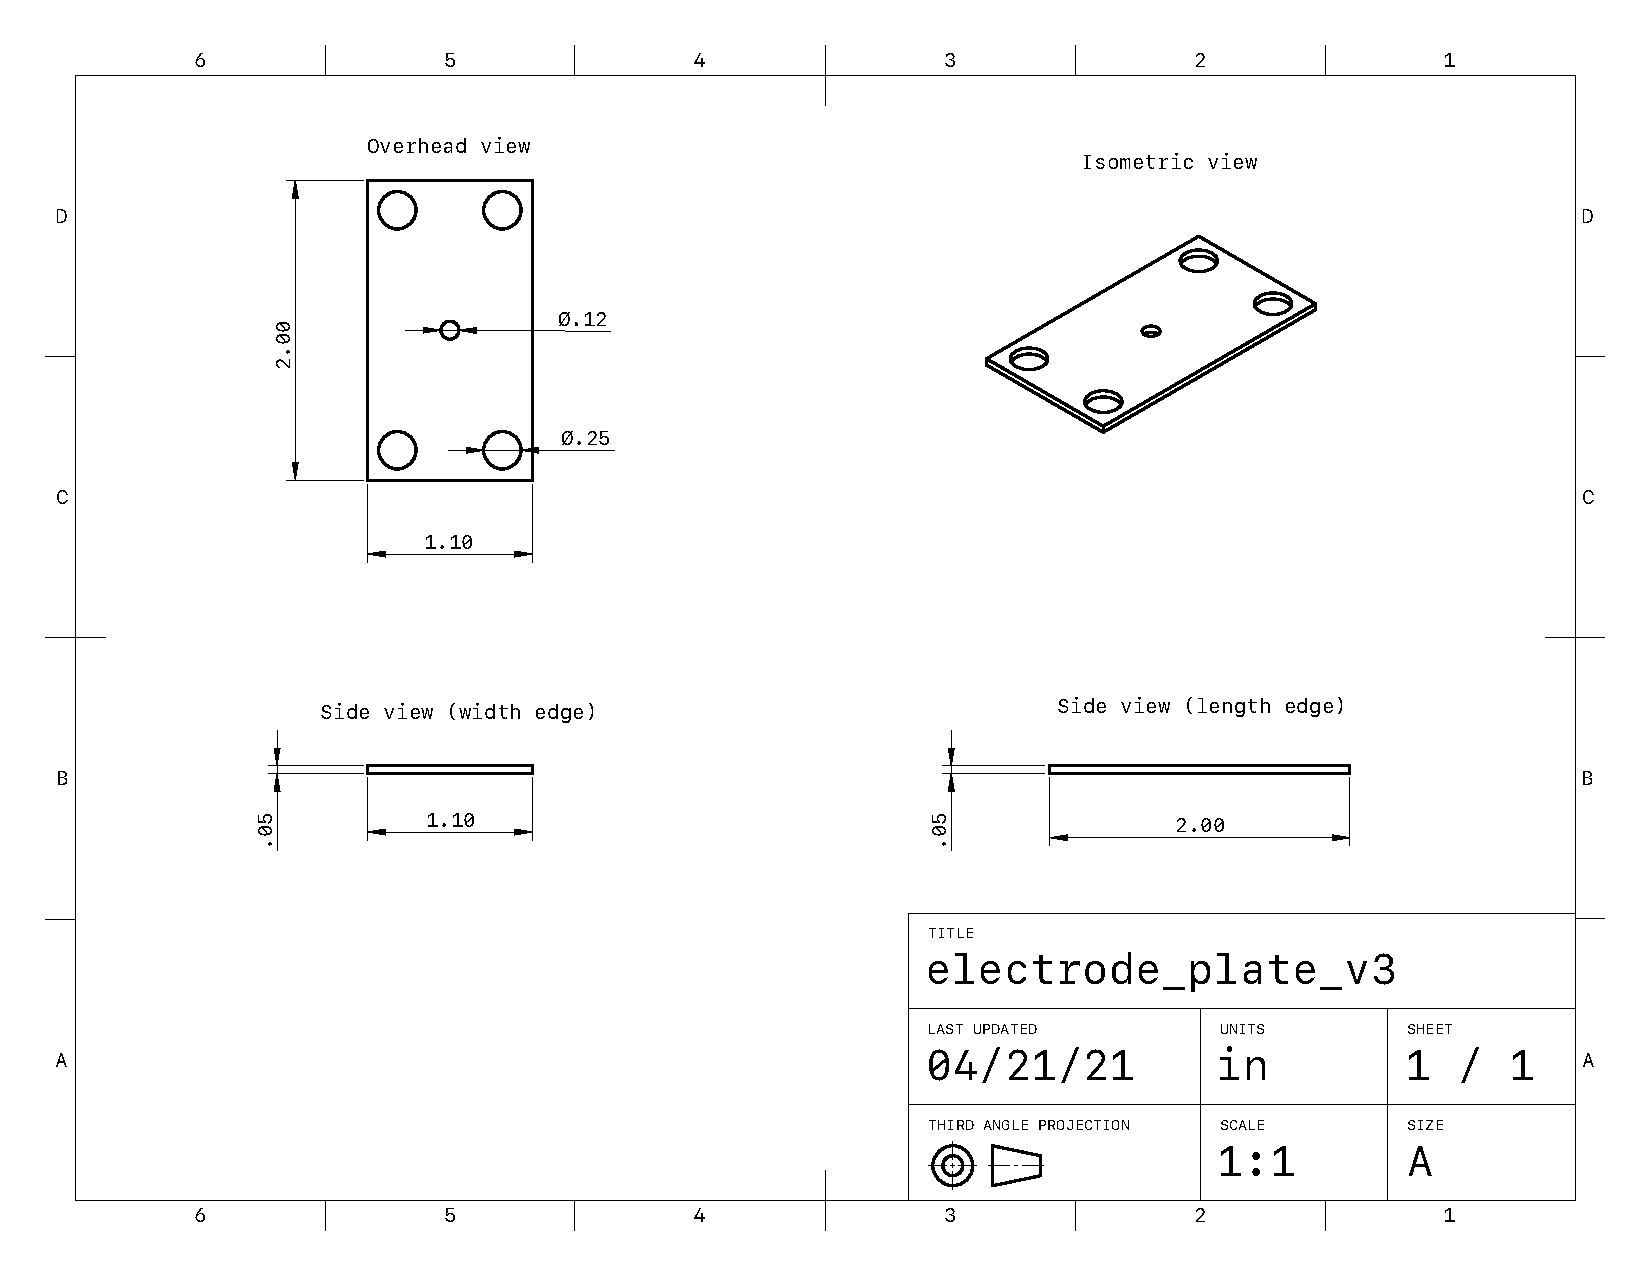
\includegraphics[width=.776\textwidth]{figs/ALGAAS/assemblies/assembly2/assembly2_electrode.pdf}
  \caption{Rectangular (.05"X1.1"X2") plates made of aluminum.}
\end{figure}

\newpage
\subsubsection{Iteration 2.1}
\begin{figure}[!ht]
	\centering
	\begin{subcaptiongroup}
		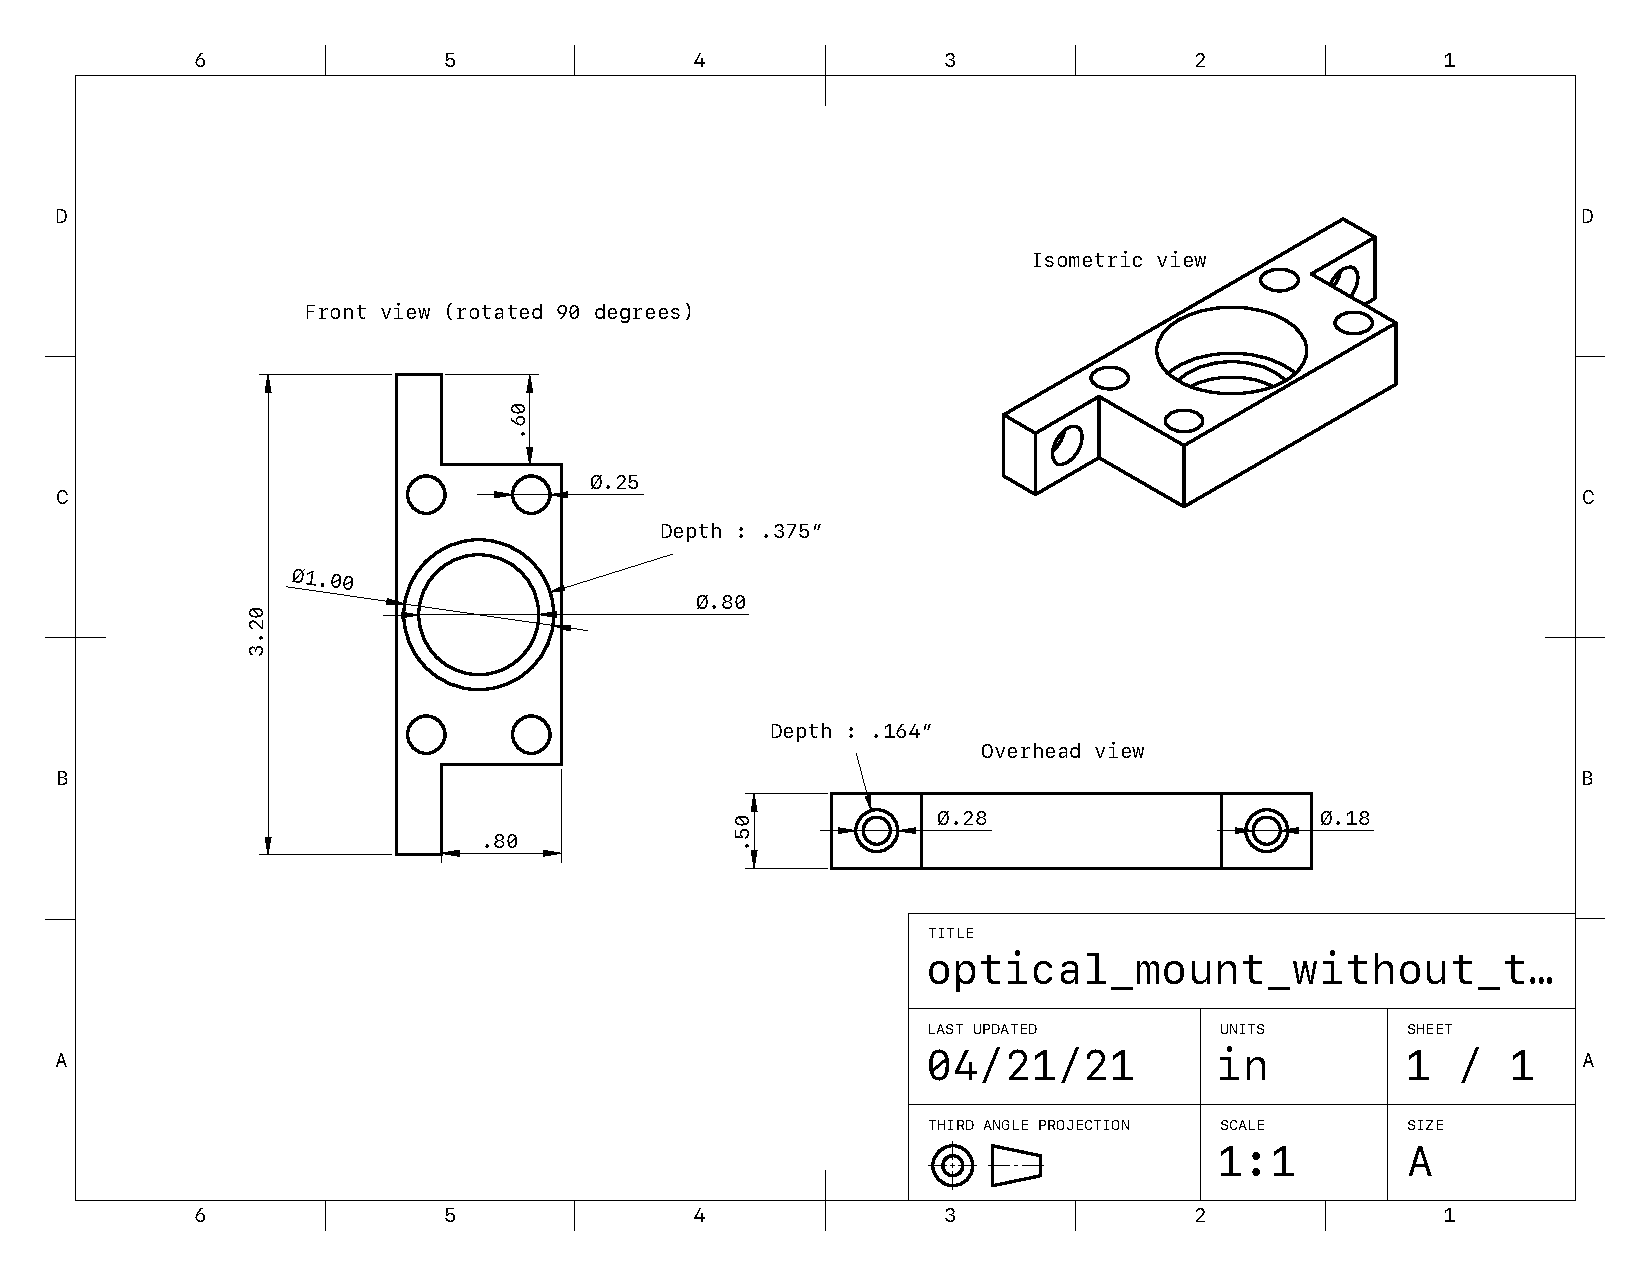
\includegraphics[width=.76\textwidth]{figs/ALGAAS/assemblies/assembly2/assembly2_PVC_mount.pdf}
		\phantomcaption\label{A2PVCmount}
		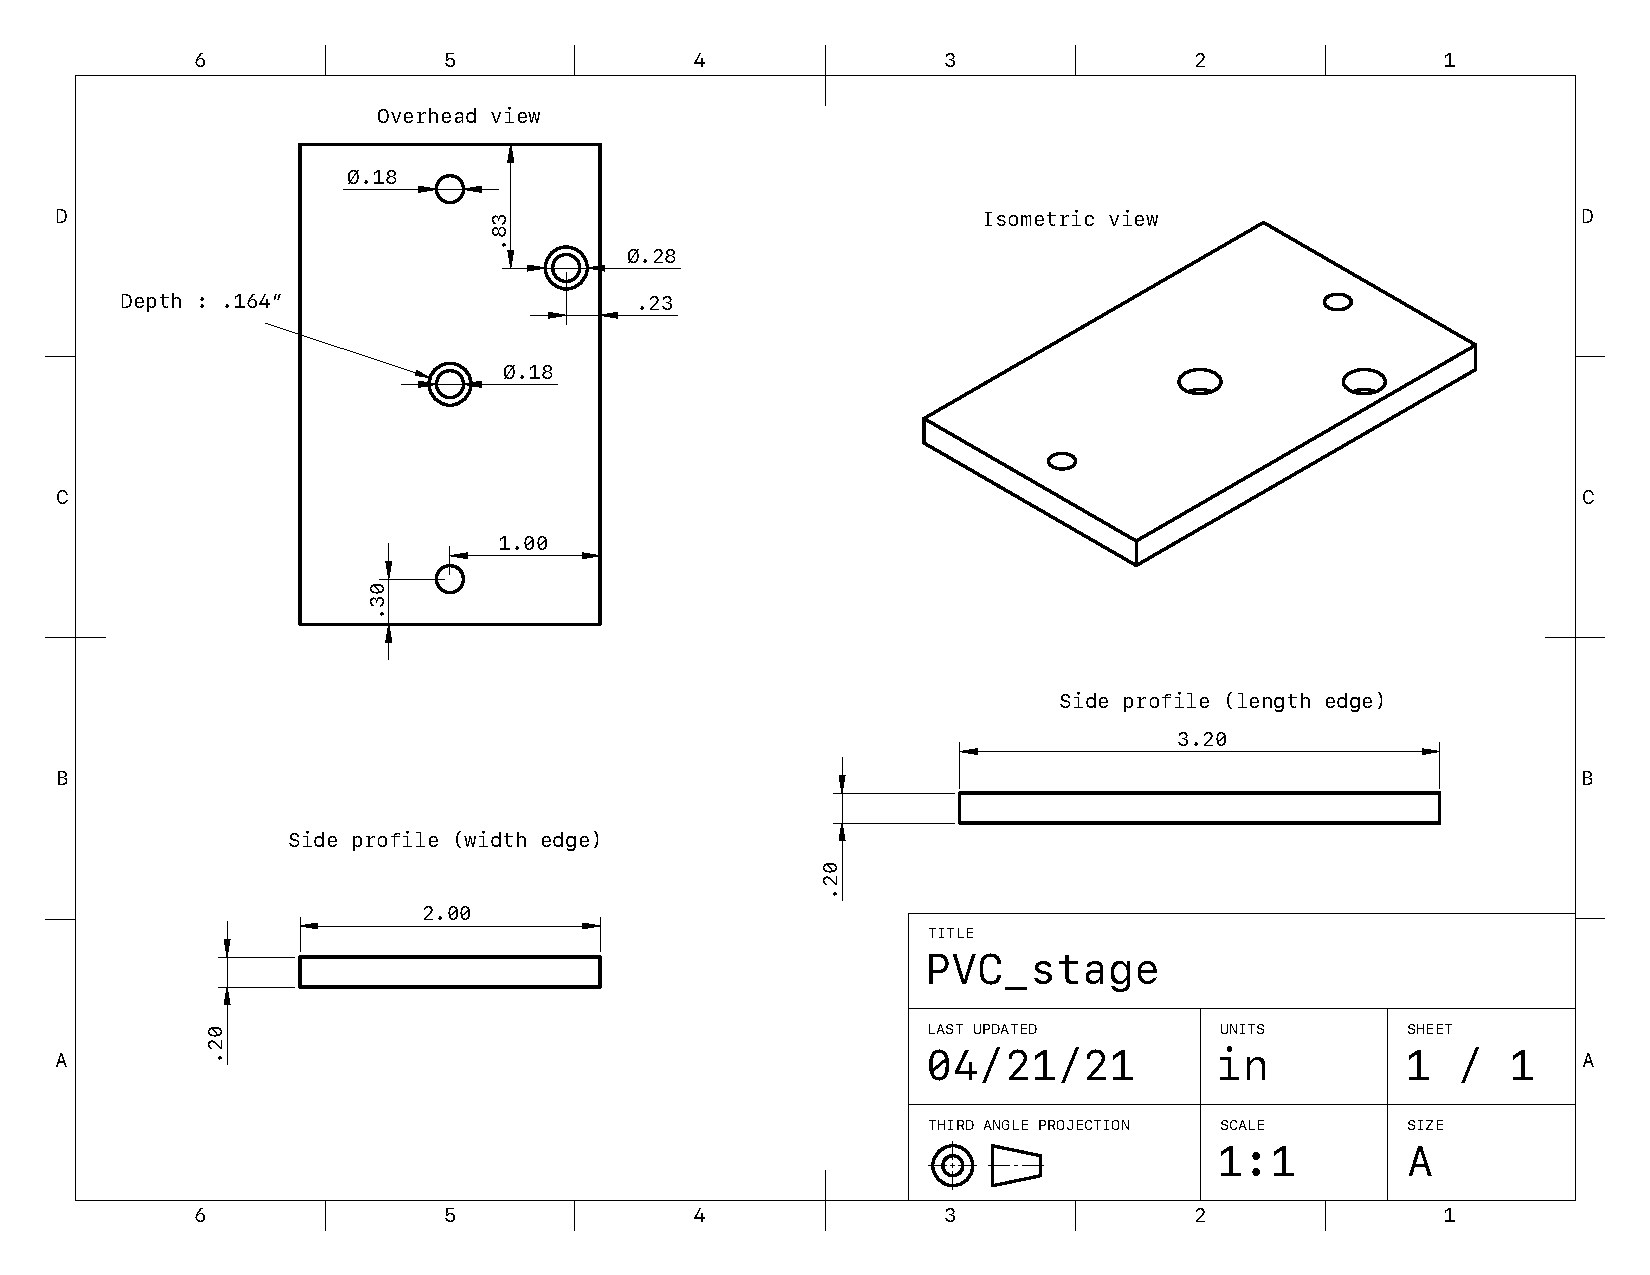
\includegraphics[width=.76\textwidth]{figs/ALGAAS/assemblies/assembly2/assembly2_PVC_stage.pdf}
		\phantomcaption\label{A2PVCstage}
	\end{subcaptiongroup}
	\caption{A design iteration of the assembly 2 mounts. Materials tried varied from PVC, PLA, and PETG. Quarter inch holes are bored in order to pass nylon screws holding electrode plates fixed to the mount.}
	\label{fig:assembly2bp}
\end{figure}
\FloatBarrier

\subsubsection{Iteration 2.2}

\subsubsection{3D printed w/ MACOR spacers}

\textcolor{red}{Insert blueprints}

\textcolor{red}{Insert printed results}

\newpage

\section{Assembly 3 [MACOR] (blueprint)}
\subsubsection{Cross section}
\subsubsection{Electrodes}

\subsubsection{Iteration 3.0}
\begin{figure}[H]
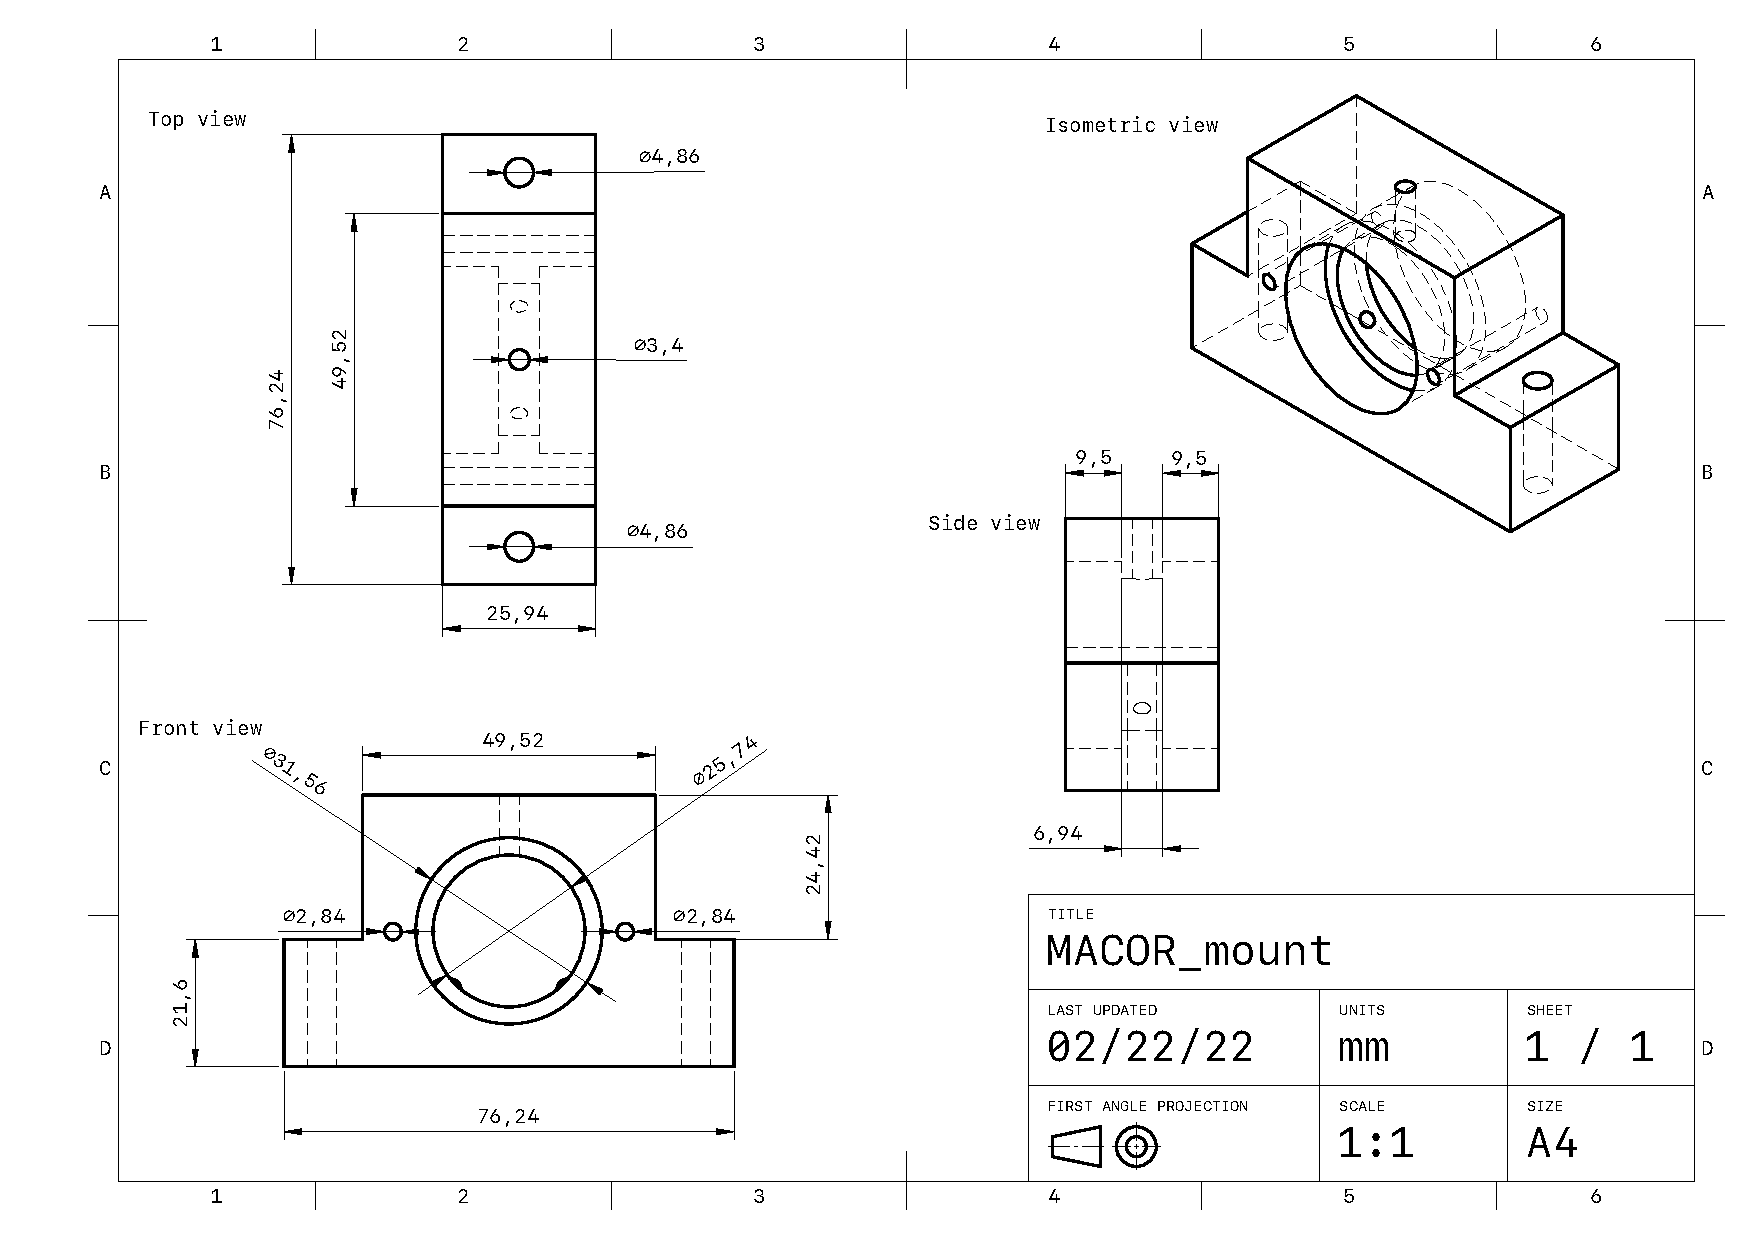
\includegraphics[width=\textwidth]{figs/ALGAAS/assemblies/assembly3/MACOR_mount.pdf}
\caption{MACOR mount design constucted in Shapr3D}
\label{fig:macormountdesign}
\end{figure}

\mbox{}
\vfill

\section{Calibration}\label{sec:calibration}
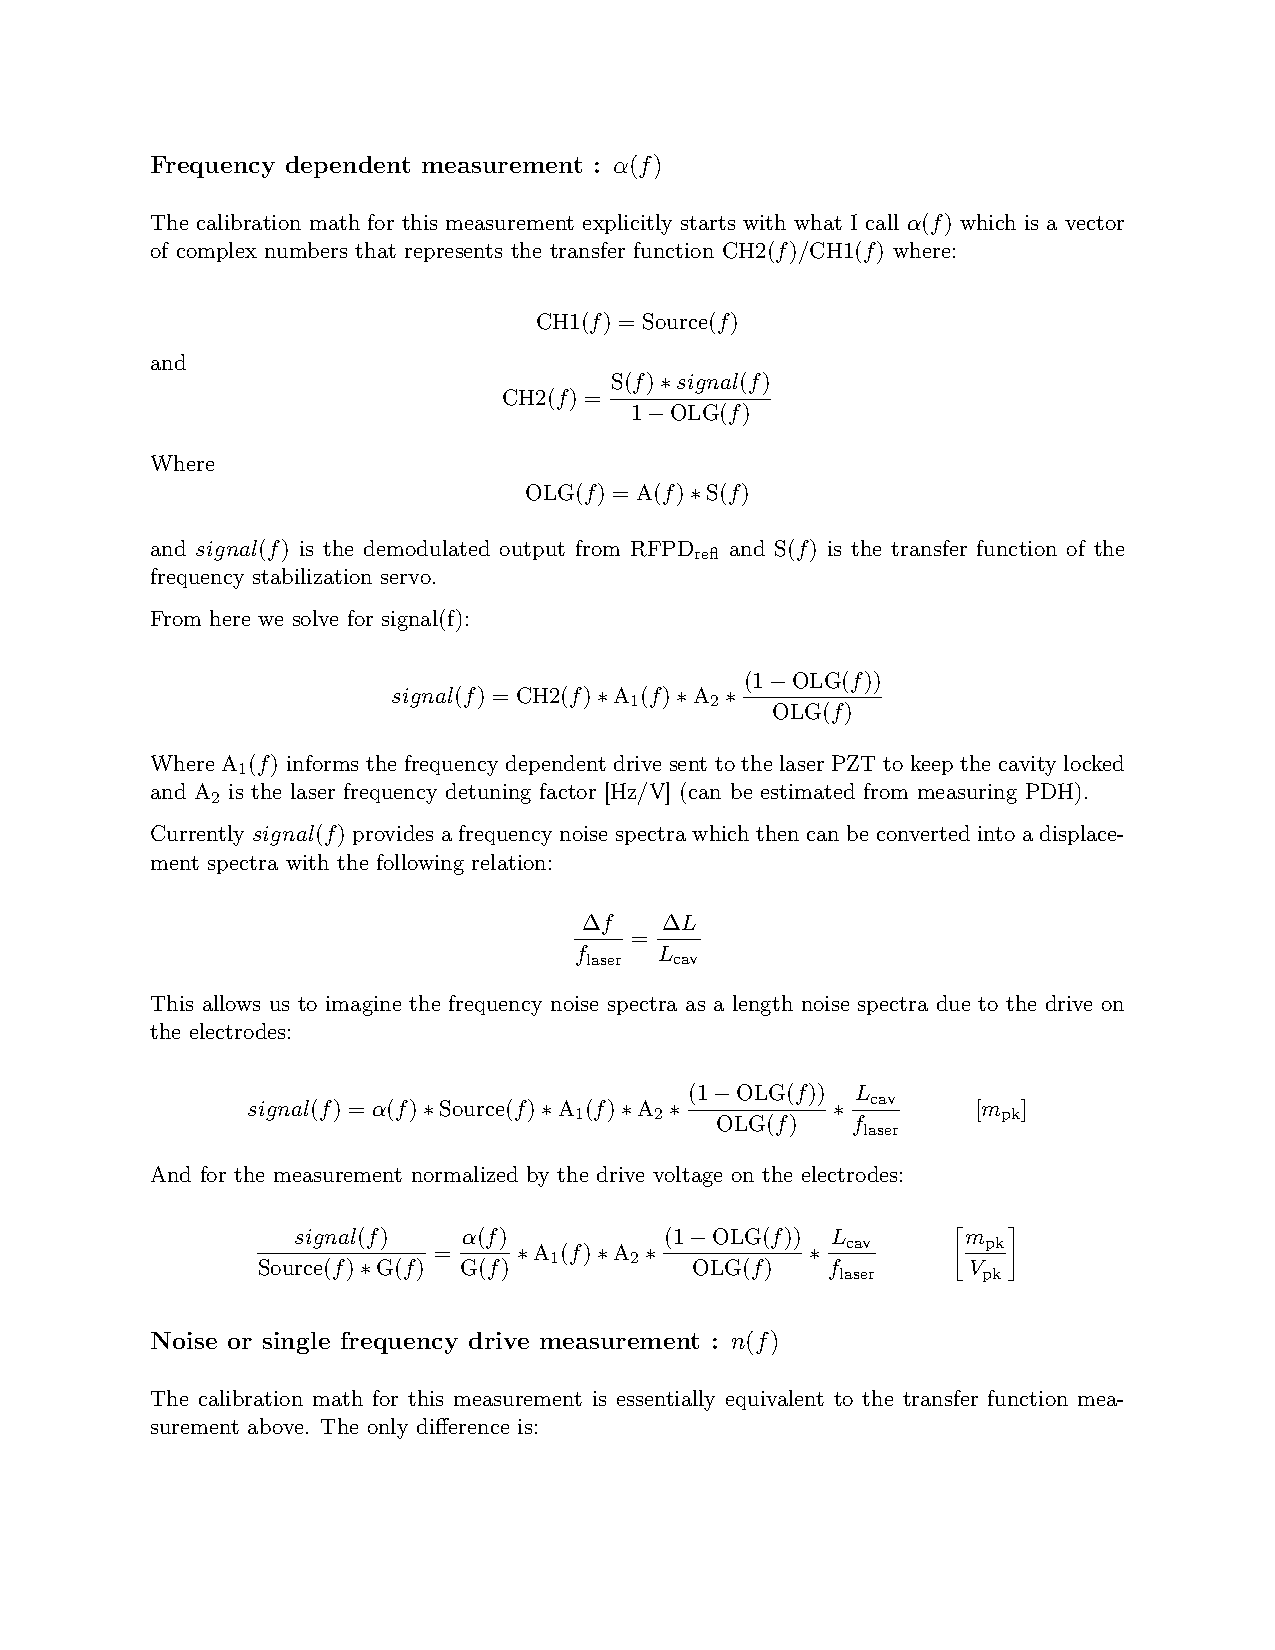
\includepdf[pages=-, pagecommand={}]{notes/pockels_calibration.pdf}

\section{Single frequency}

\section{Laplace calculator / code}

\textcolor{red}{Snippets of explicit code with a block diagram for clarity}

\section{HVA}

\section{FSS}

\begin{figure}[H]
  \begin{center}
    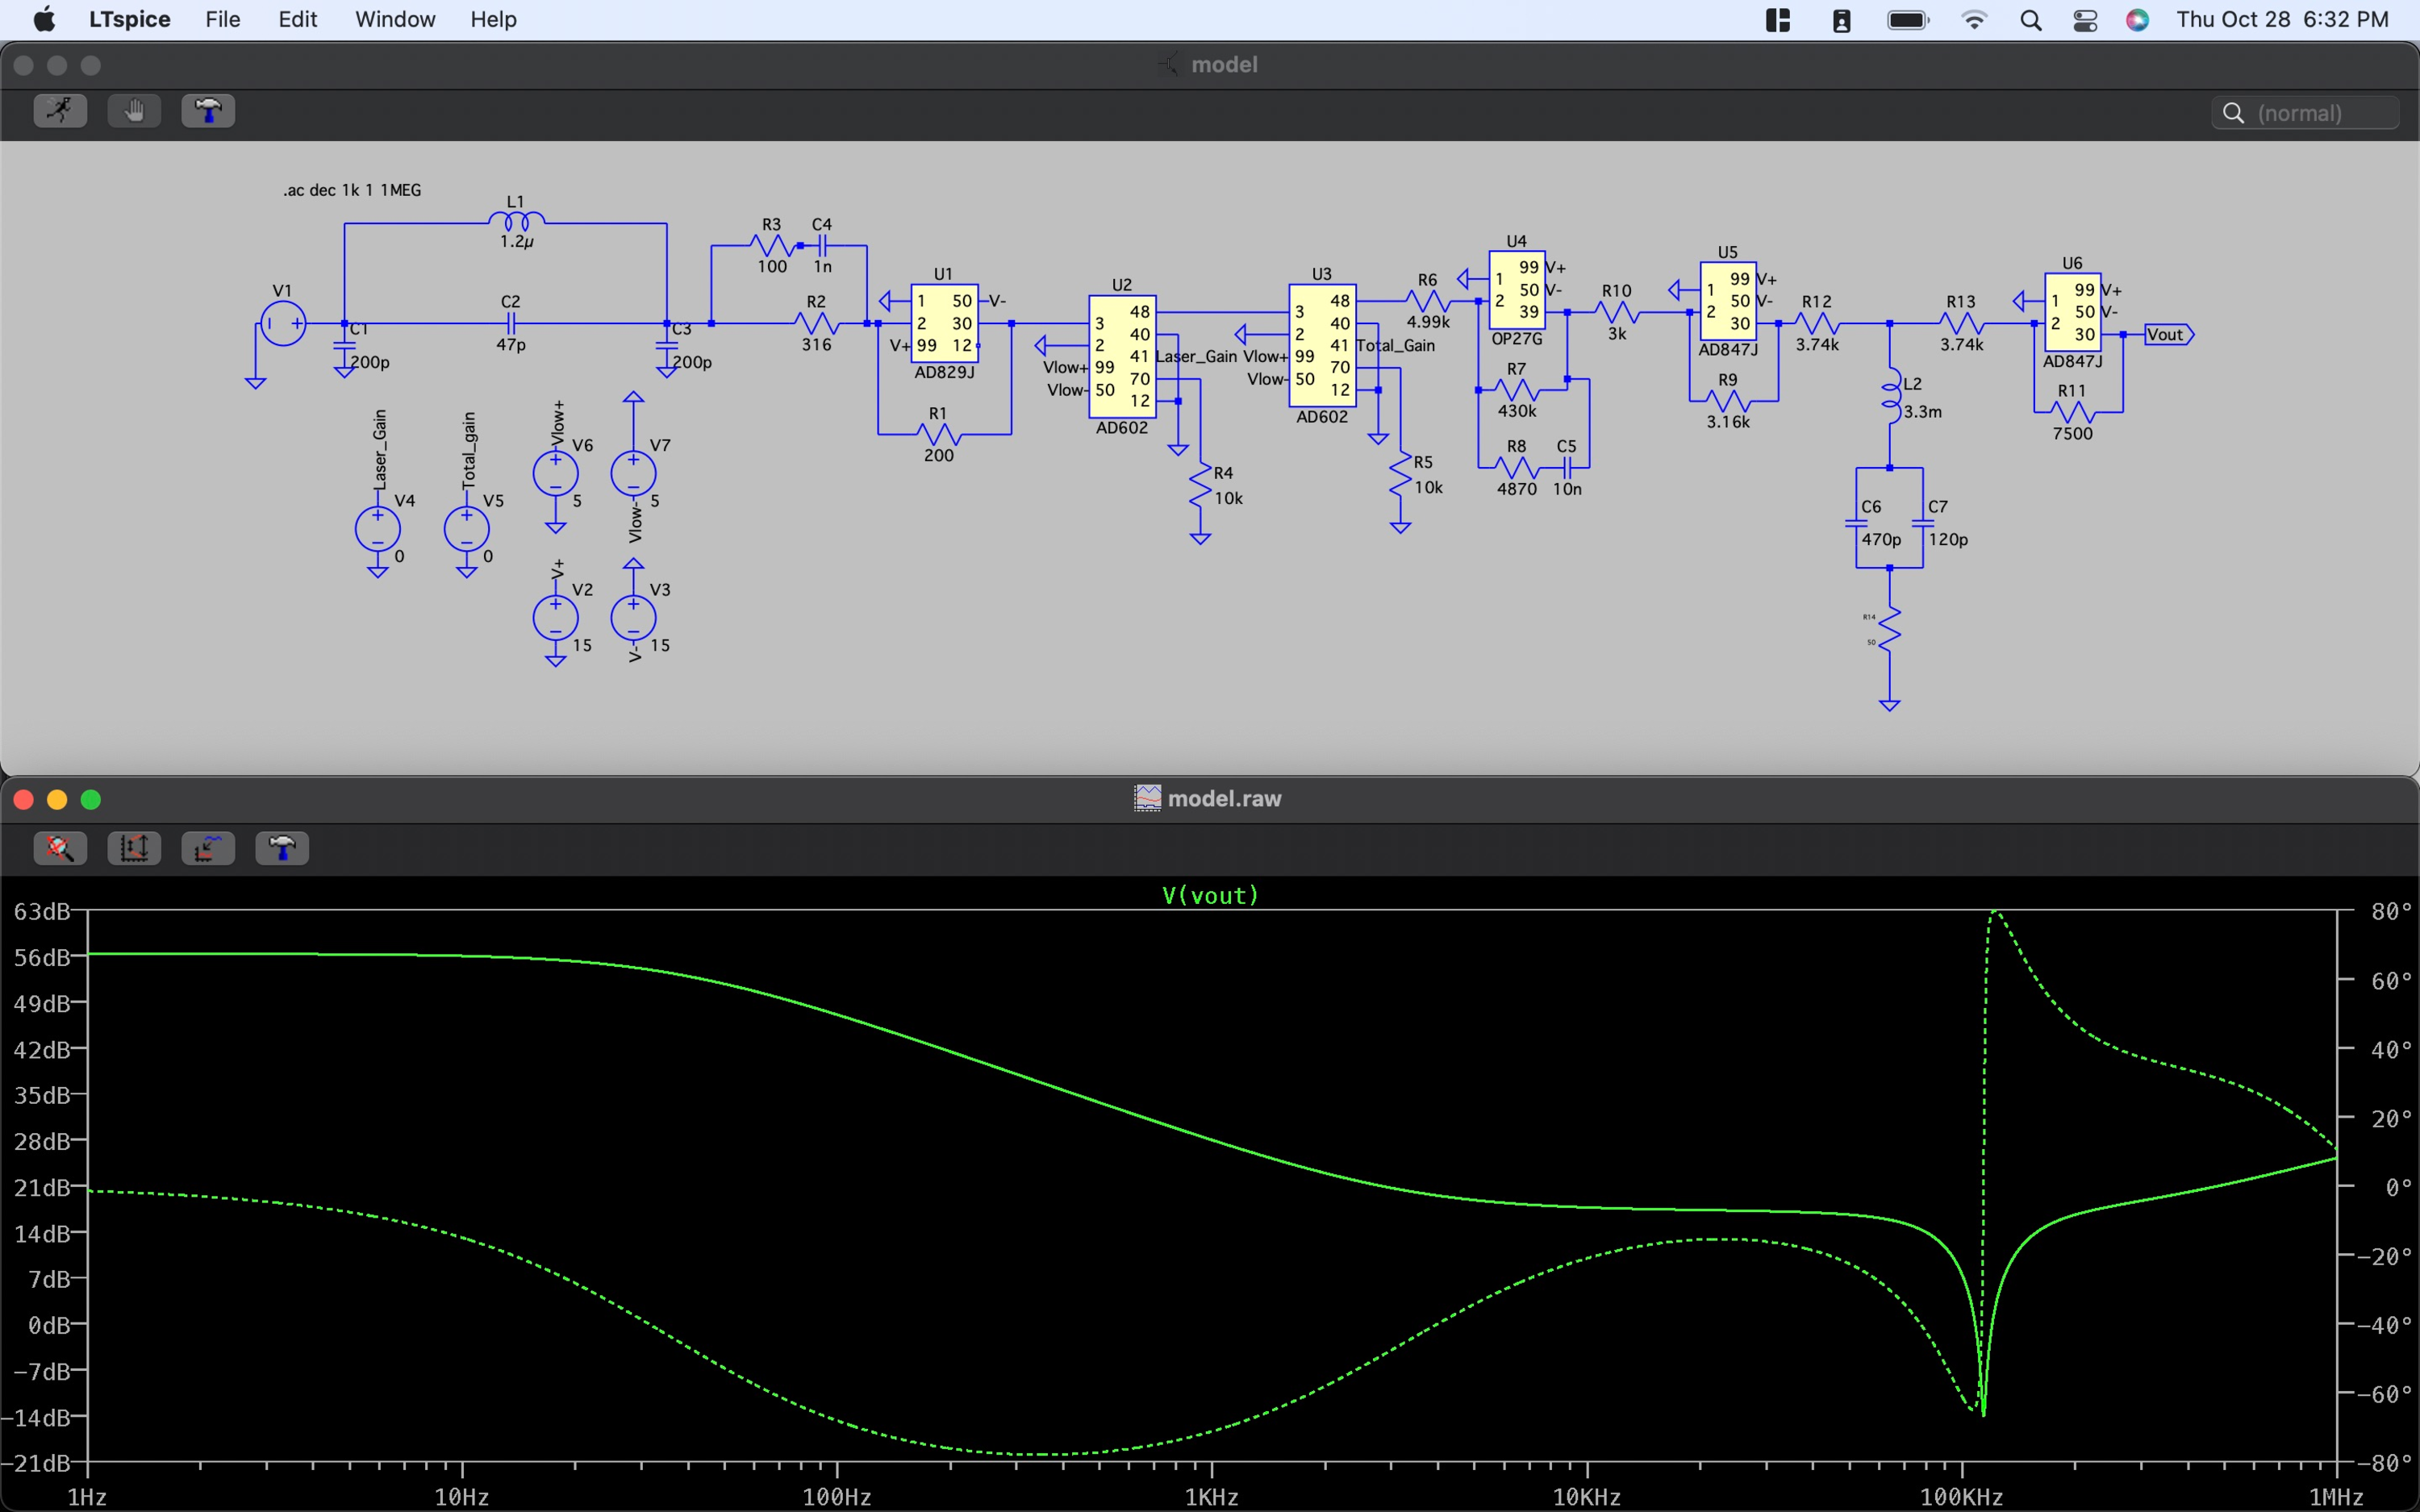
\includegraphics[width=\textwidth]{figs/ALGAAS/tfs/spice_FSS_tf.pdf}
    \caption{The FSS frequency response simulated in LTspice}
  \end{center}
  \label{fig:spiceFSS}
\end{figure}

\section{Measuring OLG [H]}

\begin{figure}[H]
  \begin{center}
    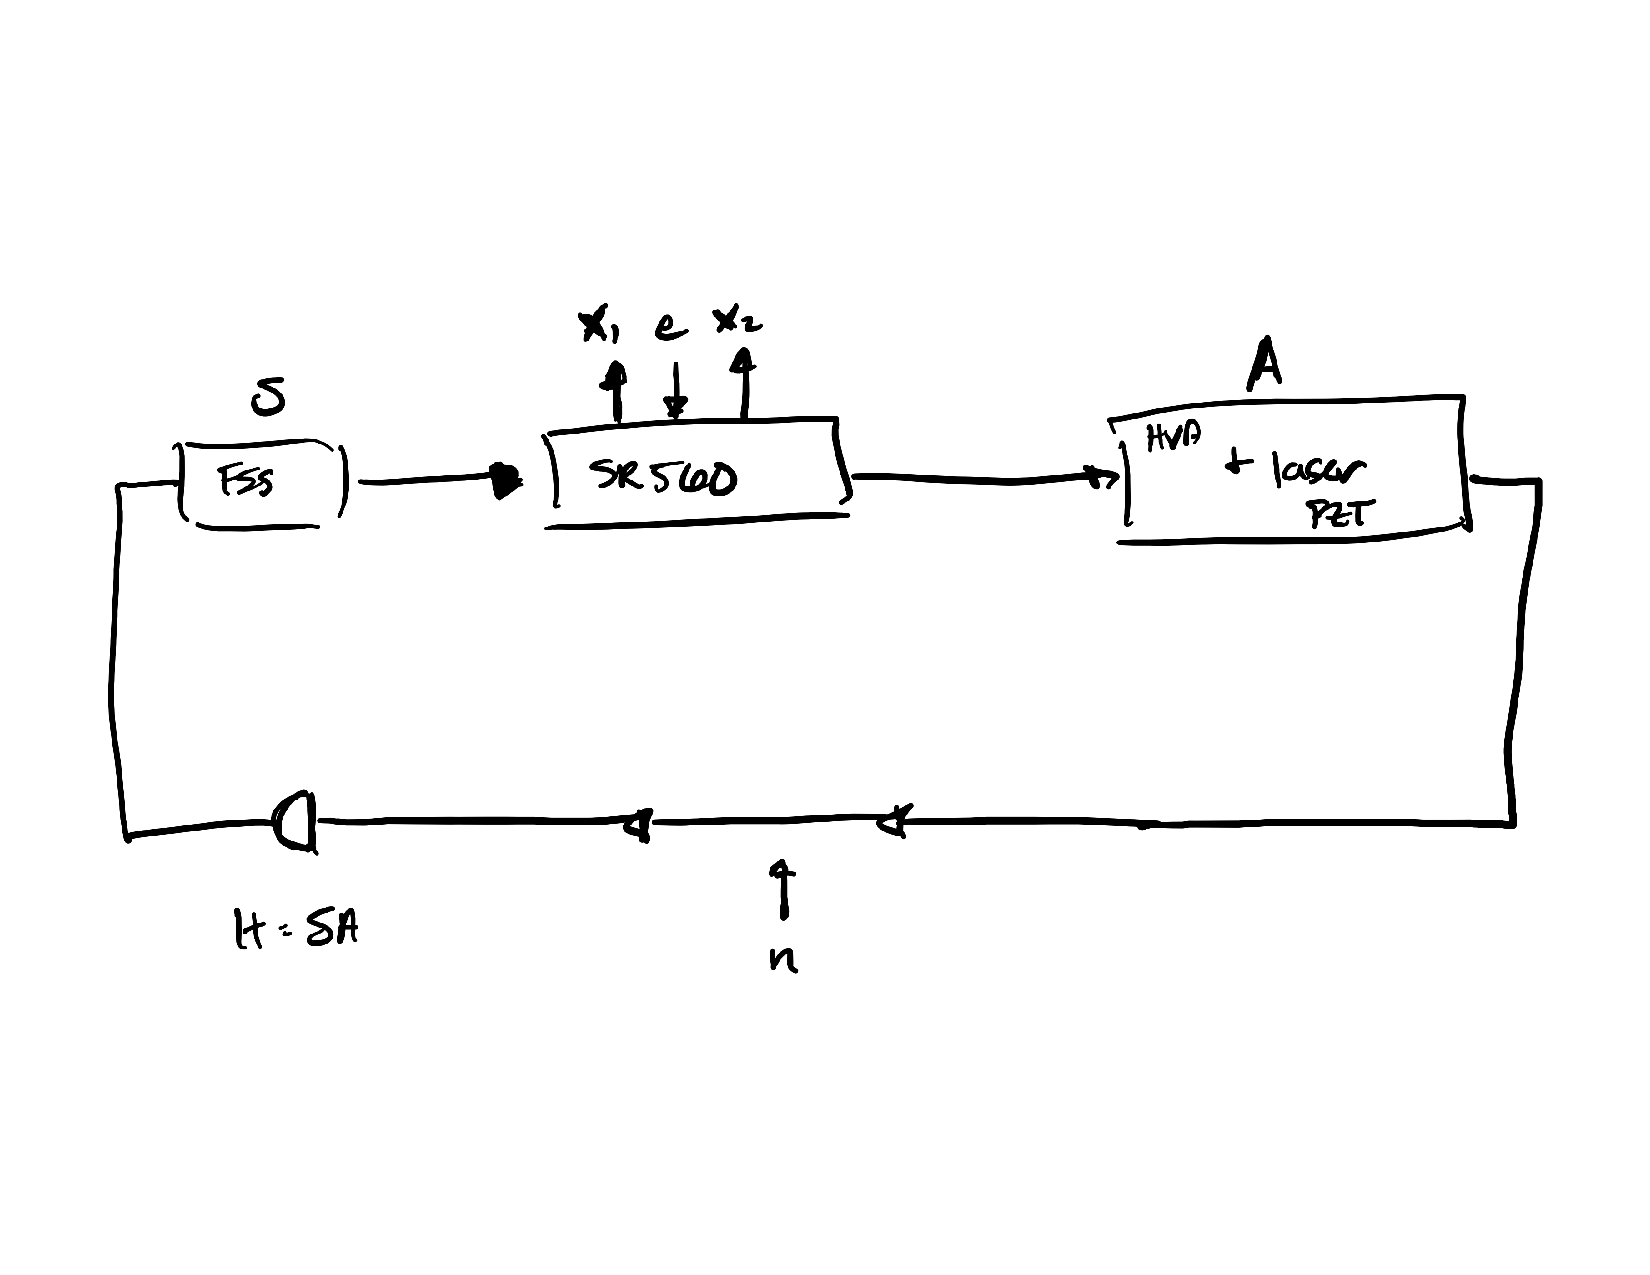
\includegraphics[width=.5\textwidth]{figs/ALGAAS/Loop_gain_measurement_drawn_diagram.pdf}
    \caption{Open loop gain measurement \textcolor{red}{drawn diagram}}
  \end{center}
  \label{fig:OLGmath}
\end{figure}

\textcolor{red}{x2 is the PSD taken immediately after the excitation point}
\begin{equation}
x_2 = e + He + H^2 e + \mathrm{H.O.T.s} = \frac{e + n}{1-H}
\end{equation}

\textcolor{red}{x1 is the PSD taken immediately prior to the excitation point}
\begin{equation}
x_1 = He + H^2e + H^3e + \mathrm{H.O.T.s}  = \frac{He}{1-H}
\end{equation}

We take the transfer function measurement $\zeta$:

\begin{equation}
\zeta = \frac{x_1}{x_2} = \frac{He/(1-H)}{(e+n)/(1-H)}
\end{equation}

Assuming the excitation is significantly larger than the noise ($e>>n$):

\begin{equation}
\zeta \approx H
\end{equation}
